\chapter{Ergebnisse}
\label{ergebnisse}

Im Rahmen dieses Abschnitts wird auf die Ergebnisse bei den verschiedenen \nameref{analyse:messreihen} eingegangen. Dabei werden zuerst die erzielten Latenz- und Durchsatzwerte für die Datenbanksysteme bei den verschiedenen Messreihen erläutert und anschließend miteinander verglichen. 

Unter den erzielten Latenzwerten werden neben der durchschnittlichen Latenz (Mean) der gebenchmarkten Operation auch das 25. (p25), 50. (p50), 75. (p75), 95. (p95) und 99. (p99) Perzentil aufgeführt sowie die höchste gemessene Latenz (Max.). Für den Vergleich der Ergebnisse der Datenbanksysteme werden allerdings vor allem die durchschnittlichen Latenzen (Mean) herangezogen. 

Beim Durchsatz wird allein der durchschnittliche Durchsatz abgebildet und für den Vergleich herangezogen. 

Die Darstellung und Auswertung der Messreihen erfolgt dabei in derselben Reihenfolge, wie sie bereits in \autoref{analyse:messreihen} aufgeführt werden. 

Zum Schluss findet eine umfassende Auswertung der Ergebnisse statt, wobei die Erkenntnisse aus allen Messreihen miteinbezogen werden. 

\section{Linkbench-10M-Const}
\label{ergebnisse:10m_const}
Dieser Abschnitt führt Latenz- und Durchsatzwerte auf, die im Rahmen dieser Messreihe für die Operationen der jeweiligen Datenbanksysteme Db2 Graph Beta 3, Db2 Graph V11.5.6.0 und Neo4j erzielt wurden. Die Ergebnisse, die dieser Abschnitt umfasst, wurden hierbei auf Basis eines kleineren konstant-verteilten Datensatzes erzielt. 

\subsection{Latenz}

Die \autoref{tab:latenz_10m_const:beta3} stellt dabei die Ergebnisse dar, die für Db2 Graph Beta 3 mit dem \texttt{Db2GraphOld}-Adapter gemessen wurden. In \autoref{tab:latenz_10m_const:ga} werden hingegen die gemessen Latenzen für Db2 Graph V11.5.6.0 beschrieben. In \autoref{tab:latenz_10m_const:ga} werden die Latenzergebnisse für Db2 Graph V11.5.6.0 aufgeführt, die bei den Messungen dieser Messreihe erzielt wurden. Die Latenzen die für Neo4j in dieser Messreihe erzielt wurden, werden in \autoref{tab:latenz_10m_const:neo4j} aufbereitet dargelegt. 

\begin{table}[!h]
\centering
\resizebox{\textwidth}{!}{
\begin{tabular}{l|r|r|r|r|r|r|r}
\hline
\rowcolor[HTML]{EFEFEF} 
\multicolumn{1}{c|}{\cellcolor[HTML]{EFEFEF}\textbf{Operation}} &
\multicolumn{1}{c|}{\cellcolor[HTML]{EFEFEF}\textbf{Mean}} &
\multicolumn{1}{c|}{\cellcolor[HTML]{EFEFEF}\textbf{p25}} &
\multicolumn{1}{c|}{\cellcolor[HTML]{EFEFEF}\textbf{p50}} &
\multicolumn{1}{c|}{\cellcolor[HTML]{EFEFEF}\textbf{p75}} &
\multicolumn{1}{c|}{\cellcolor[HTML]{EFEFEF}\textbf{p95}} &
\multicolumn{1}{c|}{\cellcolor[HTML]{EFEFEF}\textbf{p99}} &
\multicolumn{1}{c}{\cellcolor[HTML]{EFEFEF}\textbf{Max.}} \\ \hline
getNode & 6,16ms & {[}4,5{]}ms & {[}5,6{]}ms & {[}7,8{]}ms & {[}10,11{]}ms & {[}15,16{]}ms & 10.213,70ms \\
getLink & 7,79ms & {[}5,6{]}ms & {[}7,8{]}ms & {[}9,10{]}ms & {[}12,13{]}ms & {[}19,20{]}ms & 917,72ms \\
countLink & 10,72ms & {[}8,9{]}ms & {[}10,11{]}ms & {[}12,13{]}ms & {[}16,17{]}ms & {[}23,24{]}ms & 448,41ms \\
getLinkList & 10,83ms & {[}8,9{]}ms & {[}10,11{]}ms & {[}12,13{]}ms & {[}17,18{]}ms & {[}23,24{]}ms & 409,11ms \\ \hline
\end{tabular}
}
\caption{Latenz Linkbench-10M-Const Db2 Graph Beta 3}
\label{tab:latenz_10m_const:beta3}
\end{table}

\begin{table}[!h]
\centering
\resizebox{\textwidth}{!}{
\begin{tabular}{l|r|r|r|r|r|r|r}
\hline
\rowcolor[HTML]{EFEFEF} 
\multicolumn{1}{c|}{\cellcolor[HTML]{EFEFEF}\textbf{Operation}} &
\multicolumn{1}{c|}{\cellcolor[HTML]{EFEFEF}\textbf{Mean}} &
\multicolumn{1}{c|}{\cellcolor[HTML]{EFEFEF}\textbf{p25}} &
\multicolumn{1}{c|}{\cellcolor[HTML]{EFEFEF}\textbf{p50}} &
\multicolumn{1}{c|}{\cellcolor[HTML]{EFEFEF}\textbf{p75}} &
\multicolumn{1}{c|}{\cellcolor[HTML]{EFEFEF}\textbf{p95}} &
\multicolumn{1}{c|}{\cellcolor[HTML]{EFEFEF}\textbf{p99}} &
\multicolumn{1}{c}{\cellcolor[HTML]{EFEFEF}\textbf{Max.}} \\ \hline
getNode & 17,67ms & {[}4,5{]}ms & {[}12,13{]}ms & {[}29,30{]}ms & {[}42,43{]}ms & {[}47,48{]}ms & 594,61ms \\
getLink & 20,34ms & {[}6,7{]}ms & {[}14,15{]}ms & {[}32,33{]}ms & {[}48,49{]}ms & {[}56,57{]}ms & 882,82ms \\
countLink & 19,17ms & {[}5,6{]}ms & {[}13,14{]}ms & {[}31,32{]}ms & {[}46,47{]}ms & {[}53,54{]}ms & 1.109,48ms \\
getLinkList & 21,24ms & {[}6,7{]}ms & {[}14,15{]}ms & {[}34,35{]}ms & {[}50,51{]}ms & {[}58,59{]}ms & 760,85ms \\ \hline
\end{tabular}
}
\caption{Latenz Linkbench-10M-Const Db2 Graph V11.5.6.0}
\label{tab:latenz_10m_const:ga}
\end{table}

\begin{table}[!h]
\centering
\resizebox{\textwidth}{!}{
\begin{tabular}{l|r|r|r|r|r|r|r}
\hline
\rowcolor[HTML]{EFEFEF} 
\multicolumn{1}{c|}{\cellcolor[HTML]{EFEFEF}\textbf{Operation}} &
\multicolumn{1}{c|}{\cellcolor[HTML]{EFEFEF}\textbf{Mean}} &
\multicolumn{1}{c|}{\cellcolor[HTML]{EFEFEF}\textbf{p25}} &
\multicolumn{1}{c|}{\cellcolor[HTML]{EFEFEF}\textbf{p50}} &
\multicolumn{1}{c|}{\cellcolor[HTML]{EFEFEF}\textbf{p75}} &
\multicolumn{1}{c|}{\cellcolor[HTML]{EFEFEF}\textbf{p95}} &
\multicolumn{1}{c|}{\cellcolor[HTML]{EFEFEF}\textbf{p99}} &
\multicolumn{1}{c}{\cellcolor[HTML]{EFEFEF}\textbf{Max.}} \\ \hline
getNode & 2,71ms & {[}2,3{]}ms & {[}2,3{]}ms & {[}3,4{]}ms & {[}3,4{]}ms & {[}4,5{]}ms & 2.129,82ms \\
getLink & 2,87ms & {[}2,3{]}ms & {[}2,3{]}ms & {[}3,4{]}ms & {[}3,4{]}ms & {[}4,5{]}ms & 1.767,05ms \\
countLink & 2,75ms & {[}2,3{]}ms & {[}2,3{]}ms & {[}3,4{]}ms & {[}3,4{]}ms & {[}4,5{]}ms & 1.273,21ms \\
getLinkList & 2,83ms & {[}2,3{]}ms & {[}2,3{]}ms & {[}3,4{]}ms & {[}3,4{]}ms & {[}4,5{]}ms & 1.059,13ms \\ \hline
\end{tabular}
}
\caption{Latenz Linkbench-10M-Const Neo4j}
\label{tab:latenz_10m_const:neo4j}
\end{table}

Werden die Latenzergebnisse für Db2 Graph Beta 3, V11.5.6.0 und Neo4j aus den Tabellen verglichen, so fällt auf das Neo4j mit großem Abstand die geringsten Latenzwerte und somit auch die höchste Performance aufweist. Das Datenbanksystem benötigt im Schnitt ca. 2,8 Millisekunden bei für die Durchführung aller Operationen. So kann Neo4j je nach Operationsart zwei bis vier Operationen in einer Zeitspanne verarbeiten, in der Db2 Graph Beta 3 lediglich eine Operation bewältigt. Db2 Graph V11.5.6.0 weist dabei mit großem Abstand die höchste Latenz und damit die schlechteste Performance aller gebenchmarkten Datenbanksysteme auf. Es benötigt hierfür zwischen 17,67 und 21,24 Millisekunden für die Operationen im Durchschnitt. Db2 Graph bewegt sich mit einer durchschnittlichen Latenz von 6,16 bis 10,83 Millisekunden im Mittelfeld zwischen Neo4j und Db2 Graph V11.5.6.0.

Bei genauerer Betrachtung der durchschnittlichen Latenzergebnisse fällt darüber hinaus auf, dass bei Db2 Graph V11.5.6.0 und Neo4j die Operationen nach geringster Latenz geordnet die folgende Reihenfolge ergeben:
\begin{enumerate}
    \item \texttt{getNode}
    \item \texttt{countLink}
    \item \texttt{getLink}
    \item \texttt{getLinkList}
\end{enumerate}
Bei Db2 Graph Beta 3 scheint dies interessanterweise nicht der Fall zu sein. Dort weisen zwar \texttt{getNode} und \texttt{getLinkList} dieselben Positionen im Ranking auf, allerdings verfügt hier \texttt{getLink} über eine geringere Performance als \texttt{countLink}.

\subsection{Durchsatz}
Die Ergebnisse für durchschnittlichen Durchsatz zeigen ein ähnliches Bild wie die Latenzwerte der Datenbanksysteme. So ist auch in \autoref{fig:durchsatz:linkbench_10m_const} erkennbar, dass Neo4j mit Abstand den höchsten Durchsatz aufweist, gefolgt von Db2 Graph Beta 3 und dann mit etwas größerem Abstand Db2 Graph V11.5.6.0. Dabei gilt es zu beachten, dass -- anders als bei der Latenz -- beim Durchsatz ein hoher Wert auf eine hohe Performance eines Datenbanksystems hindeutet. Schließlich bedeutet ein hoher Latenzwert, dass ein Datenbanksystem dazu in der Lage ist viele Operationen pro Sekunde zu verarbeiten.  

\begin{figure}[!ht]
    \centering
    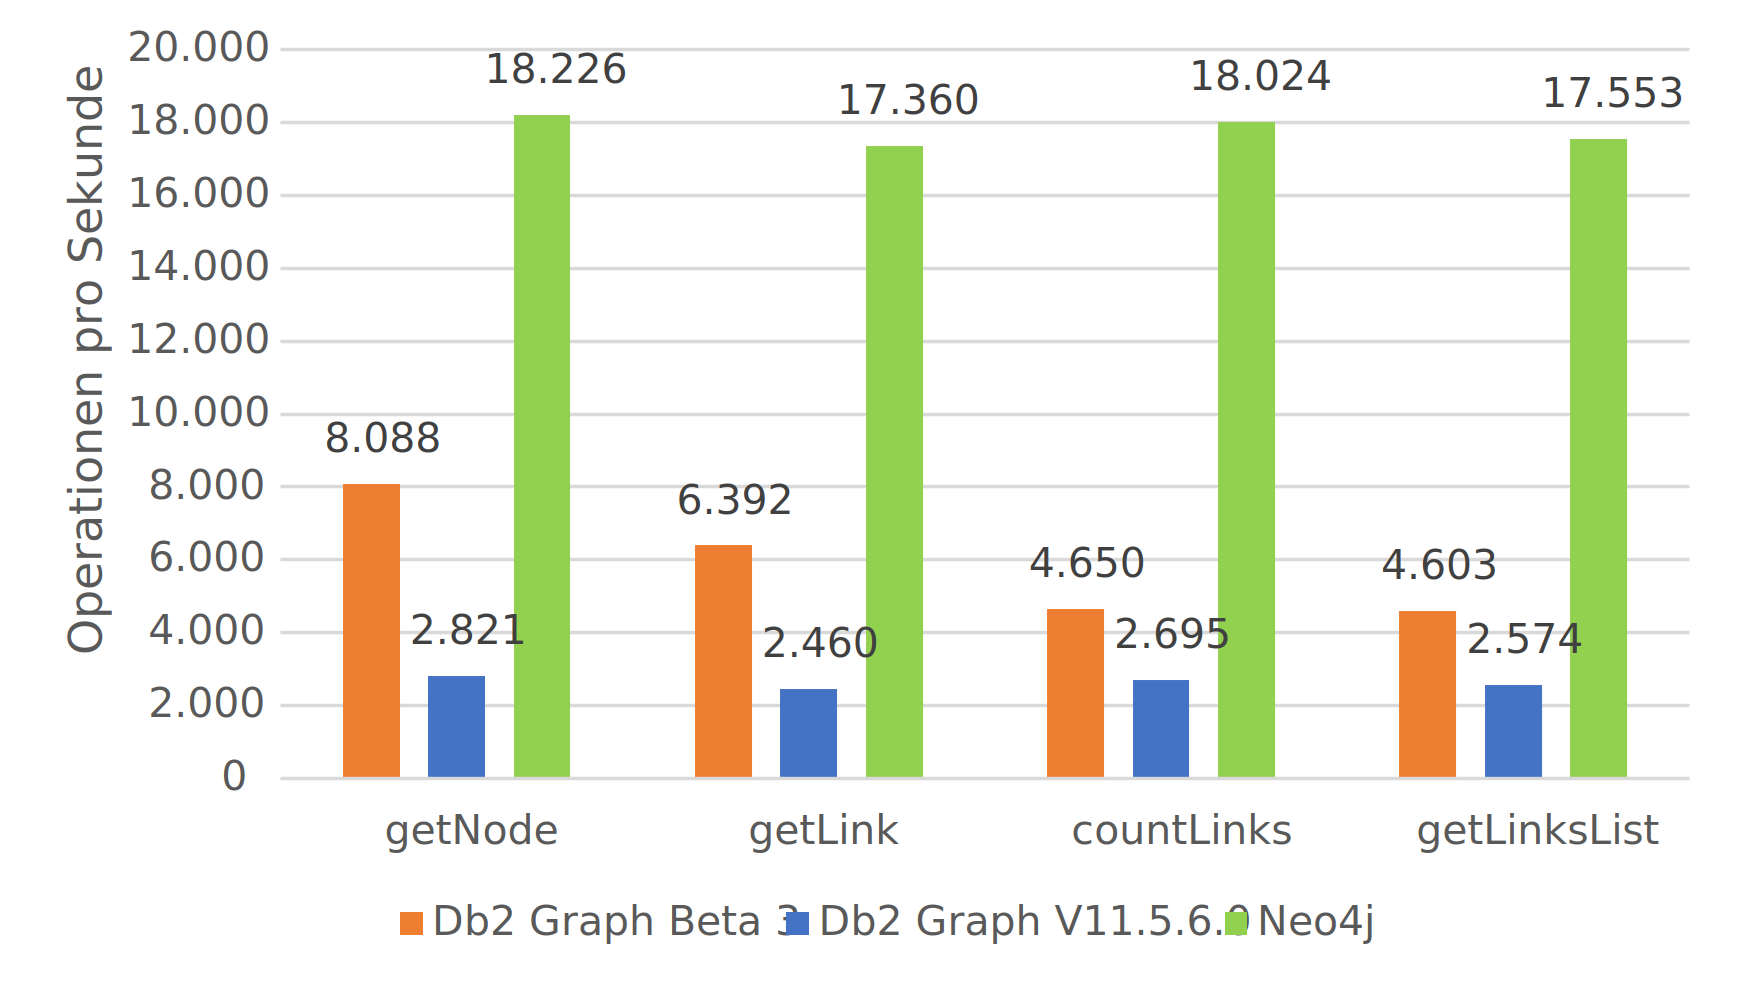
\includegraphics[width=\textwidth]{images/diagramme/linkbench_10m_const_durchsatz.pdf}
    \caption{Ergebnisse Durchsatz Linkbench-10M-Const}
    \label{fig:durchsatz:linkbench_10m_const}
\end{figure}

\section{Linkbench-10M-Const-ID}
\label{ergebnisse:10m_const_id}
In diesem Abschnitt wird auf die Messergebnisse für die Datenbanksysteme Db2 Graph Beta 3, Db2 Graph V11.5.6.0 und Neo4j eingegangen. Dafür werden die Latenz- und Durchsatzergebnisse im Folgenden dargestellt und interpretiert. 

Die Ergebnisse dieser Messreihe spielen als einzige Ergebnisse, die unter Nutzung der ID-Queries statt der regulären Queries erzielt wurden, eine besondere Rolle. So wird hier am Ende auch ein kurzer Vergleich zu den Ergebnissen der Messreihe \nameref{ergebnisse:10m_const} gezogen, da diese bis auf die Queries dasselbe Szenario abbildet.

\subsection{Latenz}
Bei der Analyse der Latenzergebnisse aus dieser Messreihe für Db2 Graph Beta 3 (\autoref{tab:latenz_10m_const_id:beta3}), Db2 Graph V11.5.6.0 (\autoref{tab:latenz_10m_const_id:ga}) und Neo4j (\autoref{tab:latenz_10m_const_id:neo4j}) fällt auf, dass auch hier Neo4j mit großem Abstand zu den beiden Db2 Graph Versionen die geringste Latenz aufweist. Dabei bewegen sich die Resultate und Performance-Unterschiede der Datenbanksysteme bei den gebenchmarkten Operationen in einer vergleichbaren Größenordnung wie bei der Messreihe \nameref{ergebnisse:10m_const} mit den regulären Queries. 

Die um ca. 3 - 4 Millisekunden verbesserten durchschnittlichen Latenzwerte für die Operationen \texttt{countLink} und \texttt{getLinkList} bei Db2 Graph Beta 3 stechen dabei allerdings etwas heraus. Leicht auffällig ist auch, dass sich die in \autoref{tab:latenz_10m_const_id:ga} abgebildeten Durchschnittswerte für \texttt{getLink}, \texttt{countLink} und \texttt{getLinkList} alle um ca. 1 - 2 Millisekunden im Vergleich zu \autoref{tab:latenz_10m_const_id:beta3} verbessert haben. 

So scheinen die Ergebnisse mit den ID-Queries tendenziell eine geringere Latenz aufzuweisen wie die Ergebnisse, die beim Einsatz der regulären Queries erzielt wurden. Allerdings werden die Unterschiede bei beiden Db2 Graph Versionen nicht als groß genug eingestuft, um diese Tendenz zu bestätigen. 

Die Ergebnisse von Neo4j werden hierbei nicht beachtet, weil diese vom Hauptunterschied zwischen den Queries -- der Formulierung der Gremlin-Queries -- nicht direkt betroffen sind.

\begin{table}[!h]
\centering
\resizebox{\textwidth}{!}{
\begin{tabular}{l|r|r|r|r|r|r|r}
\hline
\rowcolor[HTML]{EFEFEF} 
\multicolumn{1}{c|}{\cellcolor[HTML]{EFEFEF}\textbf{Operation}} &
\multicolumn{1}{c|}{\cellcolor[HTML]{EFEFEF}\textbf{Mean}} &
\multicolumn{1}{c|}{\cellcolor[HTML]{EFEFEF}\textbf{p25}} &
\multicolumn{1}{c|}{\cellcolor[HTML]{EFEFEF}\textbf{p50}} &
\multicolumn{1}{c|}{\cellcolor[HTML]{EFEFEF}\textbf{p75}} &
\multicolumn{1}{c|}{\cellcolor[HTML]{EFEFEF}\textbf{p95}} &
\multicolumn{1}{c|}{\cellcolor[HTML]{EFEFEF}\textbf{p99}} &
\multicolumn{1}{c}{\cellcolor[HTML]{EFEFEF}\textbf{Max.}} \\ \hline
getNode & 6,19ms & {[}4,5{]}ms & {[}5,6{]}ms & {[}7,8{]}ms & {[}10,11{]}ms & {[}14,15{]}ms & 1.016,58ms \\
getLink & 7,48ms & {[}5,6{]}ms & {[}6,7{]}ms & {[}8,9{]}ms & {[}12,13{]}ms & {[}17,18{]}ms & 560,31ms \\
countLink & 6,90ms & {[}5,6{]}ms & {[}6,7{]}ms & {[}8,9{]}ms & {[}11,12{]}ms & {[}17,18{]}ms & 572,13ms \\
getLinkList & 7,24ms & {[}5,6{]}ms & {[}6,7{]}ms & {[}8,9{]}ms & {[}12,13{]}ms & {[}18,19{]}ms & 588,42ms \\ \hline
\end{tabular}
}
\caption{Latenz Linkbench-10M-Const-ID Db2 Graph Beta 3}
\label{tab:latenz_10m_const_id:beta3}
\end{table}

\begin{table}[!h]
\centering
\resizebox{\textwidth}{!}{
\begin{tabular}{l|r|r|r|r|r|r|r}
\hline
\rowcolor[HTML]{EFEFEF} 
\multicolumn{1}{c|}{\cellcolor[HTML]{EFEFEF}\textbf{Operation}} &
\multicolumn{1}{c|}{\cellcolor[HTML]{EFEFEF}\textbf{Mean}} &
\multicolumn{1}{c|}{\cellcolor[HTML]{EFEFEF}\textbf{p25}} &
\multicolumn{1}{c|}{\cellcolor[HTML]{EFEFEF}\textbf{p50}} &
\multicolumn{1}{c|}{\cellcolor[HTML]{EFEFEF}\textbf{p75}} &
\multicolumn{1}{c|}{\cellcolor[HTML]{EFEFEF}\textbf{p95}} &
\multicolumn{1}{c|}{\cellcolor[HTML]{EFEFEF}\textbf{p99}} &
\multicolumn{1}{c}{\cellcolor[HTML]{EFEFEF}\textbf{Max.}} \\ \hline
getNode & 17,87ms & {[}4,5{]}ms & {[}13,14{]}ms & {[}29,30{]}ms & {[}42,43{]}ms & {[}48,49{]}ms & 1.153,64ms \\
getLink & 18,82ms & {[}5,6{]}ms & {[}13,14{]}ms & {[}30,31{]}ms & {[}45,46{]}ms & {[}52,53{]}ms & 760,44ms \\
countLink & 17,27ms & {[}4,5{]}ms & {[}12,13{]}ms & {[}28,29{]}ms & {[}42,43{]}ms & {[}47,48{]}ms & 1.261,38ms \\
getLinkList & 18,90ms & {[}5,6{]}ms & {[}13,14{]}ms & {[}31,32{]}ms & {[}45,46{]}ms & {[}52,53{]}ms & 591,80ms \\ \hline
\end{tabular}
}
\caption{Latenz Linkbench-10M-Const-ID Db2 Graph V11.5.6.0}
\label{tab:latenz_10m_const_id:ga}
\end{table}

\begin{table}[!h]
\centering
\resizebox{\textwidth}{!}{
\begin{tabular}{l|r|r|r|r|r|r|r}
\hline
\rowcolor[HTML]{EFEFEF} 
\multicolumn{1}{c|}{\cellcolor[HTML]{EFEFEF}\textbf{Operation}} &
\multicolumn{1}{c|}{\cellcolor[HTML]{EFEFEF}\textbf{Mean}} &
\multicolumn{1}{c|}{\cellcolor[HTML]{EFEFEF}\textbf{p25}} &
\multicolumn{1}{c|}{\cellcolor[HTML]{EFEFEF}\textbf{p50}} &
\multicolumn{1}{c|}{\cellcolor[HTML]{EFEFEF}\textbf{p75}} &
\multicolumn{1}{c|}{\cellcolor[HTML]{EFEFEF}\textbf{p95}} &
\multicolumn{1}{c|}{\cellcolor[HTML]{EFEFEF}\textbf{p99}} &
\multicolumn{1}{c}{\cellcolor[HTML]{EFEFEF}\textbf{Max.}} \\ \hline
getNode & 2,76ms & {[}2,3{]}ms & {[}2,3{]}ms & {[}3,4{]}ms & {[}3,4{]}ms & {[}4,5{]}ms & 748,76ms \\
getLink & 2,83ms & {[}2,3{]}ms & {[}2,3{]}ms & {[}3,4{]}ms & {[}3,4{]}ms & {[}4,5{]}ms & 1.334,29ms \\
countLink & 2,79ms & {[}2,3{]}ms & {[}2,3{]}ms & {[}3,4{]}ms & {[}3,4{]}ms & {[}4,5{]}ms & 1.070,52ms \\
getLinkList & 2,86ms & {[}2,3{]}ms & {[}2,3{]}ms & {[}3,4{]}ms & {[}3,4{]}ms & {[}4,5{]}ms & 901,75ms \\ \hline
\end{tabular}
}
\caption{Latenz Linkbench-10M-Const-ID Neo4j}
\label{tab:latenz_10m_const_id:neo4j}
\end{table}

\subsection{Durchsatz}
Die in \autoref{fig:durchsatz:linkbench_10m_const_id} abgebildeten Werte unterstreichen hierbei, dass bereits bei den Latenzwerten beschriebene Verhalten der Datenbanksysteme. Auch hier schneidet Neo4j durch die höchsten Durchsatzwerte am besten ab. Es weist dabei den höchsten Durchsatz aller Datenbanksysteme auf, gefolgt von Db2 Graph Beta 3 und V11.5.6.0. 

Beim Vergleich der Durchsatzergebnisse in \autoref{fig:durchsatz:linkbench_10m_const_id} mit denen aus \autoref{fig:durchsatz:linkbench_10m_const}, die auf Basis der regulären Queries erzielt wurden, lässt ebenfalls eine Tendenz zu etwas besseren Werten bei den ID-Queries erkennen.

\begin{figure}[!ht]
    \centering
    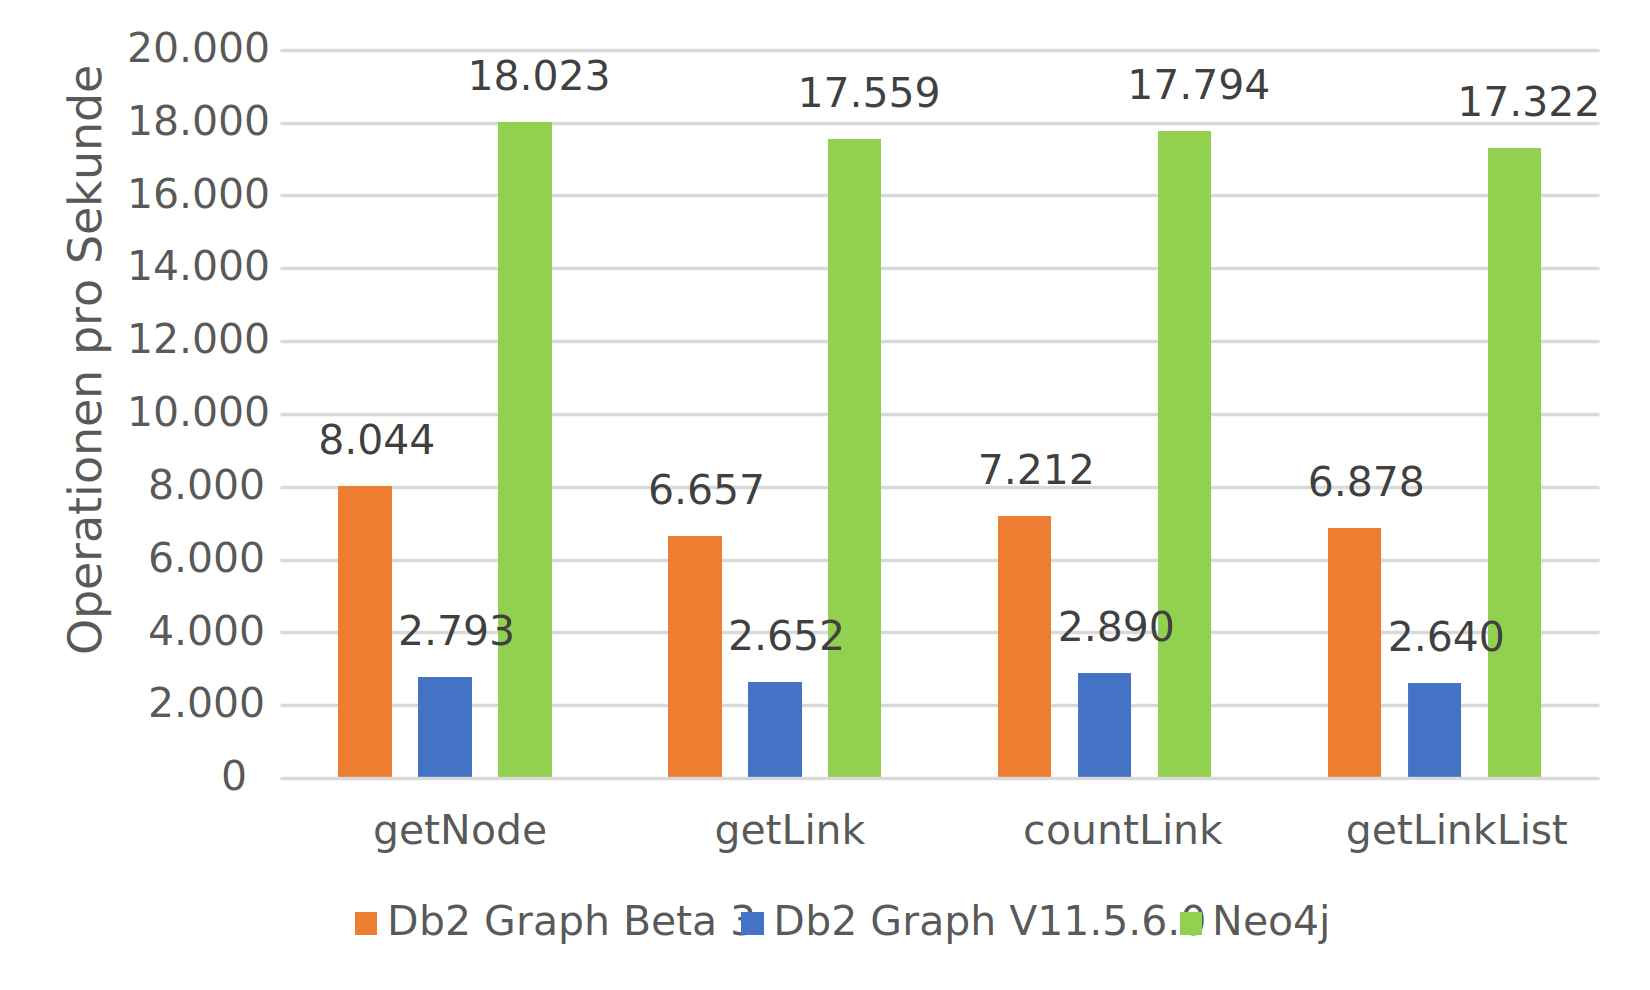
\includegraphics[width=\textwidth]{images/diagramme/linkbench_10m_const_id_durchsatz.pdf}
    \caption{Ergebnisse Durchsatz Linkbench-10M-Const-ID}
    \label{fig:durchsatz:linkbench_10m_const_id}
\end{figure}

\section{Linkbench-100M-Const}
\label{ergebnisse:100m_const}
Im Rahmen dieses Abschnitts werden die Latenz- und Durchsatzergebnisse der Messreihe \nameref{ergebnisse:100m_const} aufgeführt und mit den Ergebnissen der Messreihe \nameref{ergebnisse:10m_const} verglichen. Schließlich handelt es sich hierbei um zwei Messreihen die sich lediglich in der Größe des Datensatzes unterscheiden. Diese Messreihe verfügt hierbei um einen Datensatz, der um den Faktor-10 größer ist als der, der im Rahmen der Reihe \nameref{ergebnisse:10m_const} herangezogen wird. 

\subsection{Latenz}
Werden die in \autoref{tab:latenz_100m_const:beta3}, \autoref{tab:latenz_100m_const:ga} und \autoref{tab:latenz_100m_const:neo4j} aufgeführten Werte, die die Latenzergebnisse für Db2 Graph Beta 3, Db2 Graph V11.5.6.0 und Neo4j beinhalten, miteinander verglichen, so ergibt sich einmal mehr das Bild, dass Neo4j die geringste Latenz aller drei gebenchmarkten Datenbanksysteme aufweist. Auf Platz zwei der Datenbanksysteme mit der geringsten Latenz für die Operationen folgt dabei wieder Db2 Graph Beta 3. Es weist hierbei im Durchschnitt eine halb bis ein Drittel so hohen Latenzwert wie Db2 Graph V11.5.6.0 auf.

\begin{table}[!h]
\centering
\resizebox{\textwidth}{!}{
\begin{tabular}{l|r|r|r|r|r|r|r}
\hline
\rowcolor[HTML]{EFEFEF} 
\multicolumn{1}{c|}{\cellcolor[HTML]{EFEFEF}\textbf{Operation}} &
\multicolumn{1}{c|}{\cellcolor[HTML]{EFEFEF}\textbf{Mean}} &
\multicolumn{1}{c|}{\cellcolor[HTML]{EFEFEF}\textbf{p25}} &
\multicolumn{1}{c|}{\cellcolor[HTML]{EFEFEF}\textbf{p50}} &
\multicolumn{1}{c|}{\cellcolor[HTML]{EFEFEF}\textbf{p75}} &
\multicolumn{1}{c|}{\cellcolor[HTML]{EFEFEF}\textbf{p95}} &
\multicolumn{1}{c|}{\cellcolor[HTML]{EFEFEF}\textbf{p99}} &
\multicolumn{1}{c}{\cellcolor[HTML]{EFEFEF}\textbf{Max.}} \\ \hline
getNode & 6,34ms & {[}4,5{]}ms & {[}5,6{]}ms & {[}7,8{]}ms & {[}10,11{]}ms & {[}16,17{]}ms & 808,08ms \\
getLink & 8,22ms & {[}6,7{]}ms & {[}7,8{]}ms & {[}9,10{]}ms & {[}13,14{]}ms & {[}20,21{]}ms & 1.500,61ms \\
countLink & 10,95ms & {[}8,9{]}ms & {[}10,11{]}ms & {[}12,13{]}ms & {[}17,18{]}ms & {[}24,25{]}ms & 402,42ms \\
getLinkList & 11,24ms & {[}8,9{]}ms & {[}10,11{]}ms & {[}12,13{]}ms & {[}17,18{]}ms & {[}24,25{]}ms & 791,5ms \\ \hline
\end{tabular}
}
\caption{Latenz Linkbench-100M-Const Db2 Graph Beta 3}
\label{tab:latenz_100m_const:beta3}
\end{table}

\begin{table}[!h]
\centering
\resizebox{\textwidth}{!}{
\begin{tabular}{l|r|r|r|r|r|r|r}
\hline
\rowcolor[HTML]{EFEFEF} 
\multicolumn{1}{c|}{\cellcolor[HTML]{EFEFEF}\textbf{Operation}} &
\multicolumn{1}{c|}{\cellcolor[HTML]{EFEFEF}\textbf{Mean}} &
\multicolumn{1}{c|}{\cellcolor[HTML]{EFEFEF}\textbf{p25}} &
\multicolumn{1}{c|}{\cellcolor[HTML]{EFEFEF}\textbf{p50}} &
\multicolumn{1}{c|}{\cellcolor[HTML]{EFEFEF}\textbf{p75}} &
\multicolumn{1}{c|}{\cellcolor[HTML]{EFEFEF}\textbf{p95}} &
\multicolumn{1}{c|}{\cellcolor[HTML]{EFEFEF}\textbf{p99}} &
\multicolumn{1}{c}{\cellcolor[HTML]{EFEFEF}\textbf{Max.}} \\ \hline
getNode & 17,88ms & {[}4,5{]}ms & {[}13,14{]}ms & {[}29,30{]}ms & {[}42,43{]}ms & {[}48,49{]}ms & 680,9ms \\
getLink & 20,71ms & {[}6,7{]}ms & {[}14,15{]}ms & {[}33,34{]}ms & {[}48,49{]}ms & {[}56,57{]}ms & 1.807,64ms \\
countLink & 18,92ms & {[}5,6{]}ms & {[}13,14{]}ms & {[}30,31{]}ms & {[}45,46{]}ms & {[}52,53{]}ms & 704,75ms \\
getLinkList & 19,67ms & {[}5,6{]}ms & {[}13,14{]}ms & {[}32,33{]}ms & {[}47,48{]}ms & {[}54,55{]}ms & 3.792,33ms \\ \hline
\end{tabular}
}
\caption{Latenz Linkbench-100M-Const Db2 Graph V11.5.6.0}
\label{tab:latenz_100m_const:ga}
\end{table}

\begin{table}[!h]
\centering
\resizebox{\textwidth}{!}{
\begin{tabular}{l|r|r|r|r|r|r|r}
\hline
\rowcolor[HTML]{EFEFEF} 
\multicolumn{1}{c|}{\cellcolor[HTML]{EFEFEF}\textbf{Operation}} &
\multicolumn{1}{c|}{\cellcolor[HTML]{EFEFEF}\textbf{Mean}} &
\multicolumn{1}{c|}{\cellcolor[HTML]{EFEFEF}\textbf{p25}} &
\multicolumn{1}{c|}{\cellcolor[HTML]{EFEFEF}\textbf{p50}} &
\multicolumn{1}{c|}{\cellcolor[HTML]{EFEFEF}\textbf{p75}} &
\multicolumn{1}{c|}{\cellcolor[HTML]{EFEFEF}\textbf{p95}} &
\multicolumn{1}{c|}{\cellcolor[HTML]{EFEFEF}\textbf{p99}} &
\multicolumn{1}{c}{\cellcolor[HTML]{EFEFEF}\textbf{Max.}} \\ \hline
getNode & 2,85ms & {[}2,3{]}ms & {[}2,3{]}ms & {[}3,4{]}ms & {[}3,4{]}ms & {[}4,5{]}ms & 1.080,62ms \\
getLink & 2,99ms & {[}2,3{]}ms & {[}2,3{]}ms & {[}3,4{]}ms & {[}4,5{]}ms & {[}5,6{]}ms & 1.306,96ms \\
countLink & 2,84ms & {[}2,3{]}ms & {[}2,3{]}ms & {[}3,4{]}ms & {[}3,4{]}ms & {[}4,5{]}ms & 1.222,04ms \\
getLinkList & 2,93ms & {[}2,3{]}ms & {[}2,3{]}ms & {[}3,4{]}ms & {[}4,5{]}ms & {[}5,6{]}ms & 975,43ms \\ \hline
\end{tabular}
}
\caption{Latenz Linkbench-100M-Const Neo4j}
\label{tab:latenz_100m_const:neo4j}
\end{table}

Beim Vergleich der in diesem Abschnitt aufgeführten Latenzergebnisse, mit denen aus \nameref{ergebnisse:10m_const} die auf Basis eines kleineren Datensatzes erzielt wurden, fällt auf, dass die durchschnittliche Latenz bei allen Datenbanksystemen geringfügig höher ausfallen, als bei \nameref{ergebnisse:10m_const}. 

Dieses Verhalten entspricht dabei allerdings den Erwartungen, da normalerweise immer davon ausgegangen werden sollte, dass die Beantwortung der Queries auf Basis eines größeren Datensatzes mehr Zeit benötigt als bei einem kleinen Datensatz. Schließlich steigt hierbei der Verarbeitungsaufwand für die Datenbanksysteme. 

Der Unterschied zwischen den Messreihen fällt hier sogar kleiner aus als erwartet, was vermutlich auf den großen Bufferpool oder Page-Cache der gebenchmarkten Datenbanksysteme zurückgeführt werden kann. So sollten sowohl der Linkbench-10M als auch der Linkbench-100M Datensatz komplett in den Bufferpool oder den Page-Cache von Db2 und Neo4j passen.

\subsection{Durchsatz}
Die im Rahmen dieser Messreihe erzielten Durchsatzwerte (\autoref{fig:durchsatz:linkbench_100m_const}) unterstreichen auch bei dieser Messreihe die bei den Latenzwerten beobachteten Sachverhalte. Auch hier weist Db2 Graph V11.5.6.0 den schlechtesten beziehungsweise geringsten Wert auf und Neo4j den besten (höchsten). Auch bleiben die Durchsatzwerte alle geringfügig unterhalb der Durchsatzergebnisse aus \autoref{fig:durchsatz:linkbench_10m_const}, die auf Basis des kleineren  Datensatzes aber gleich verteilten Datensatzes ermittelt wurden. 

\begin{figure}[!ht]
    \centering
    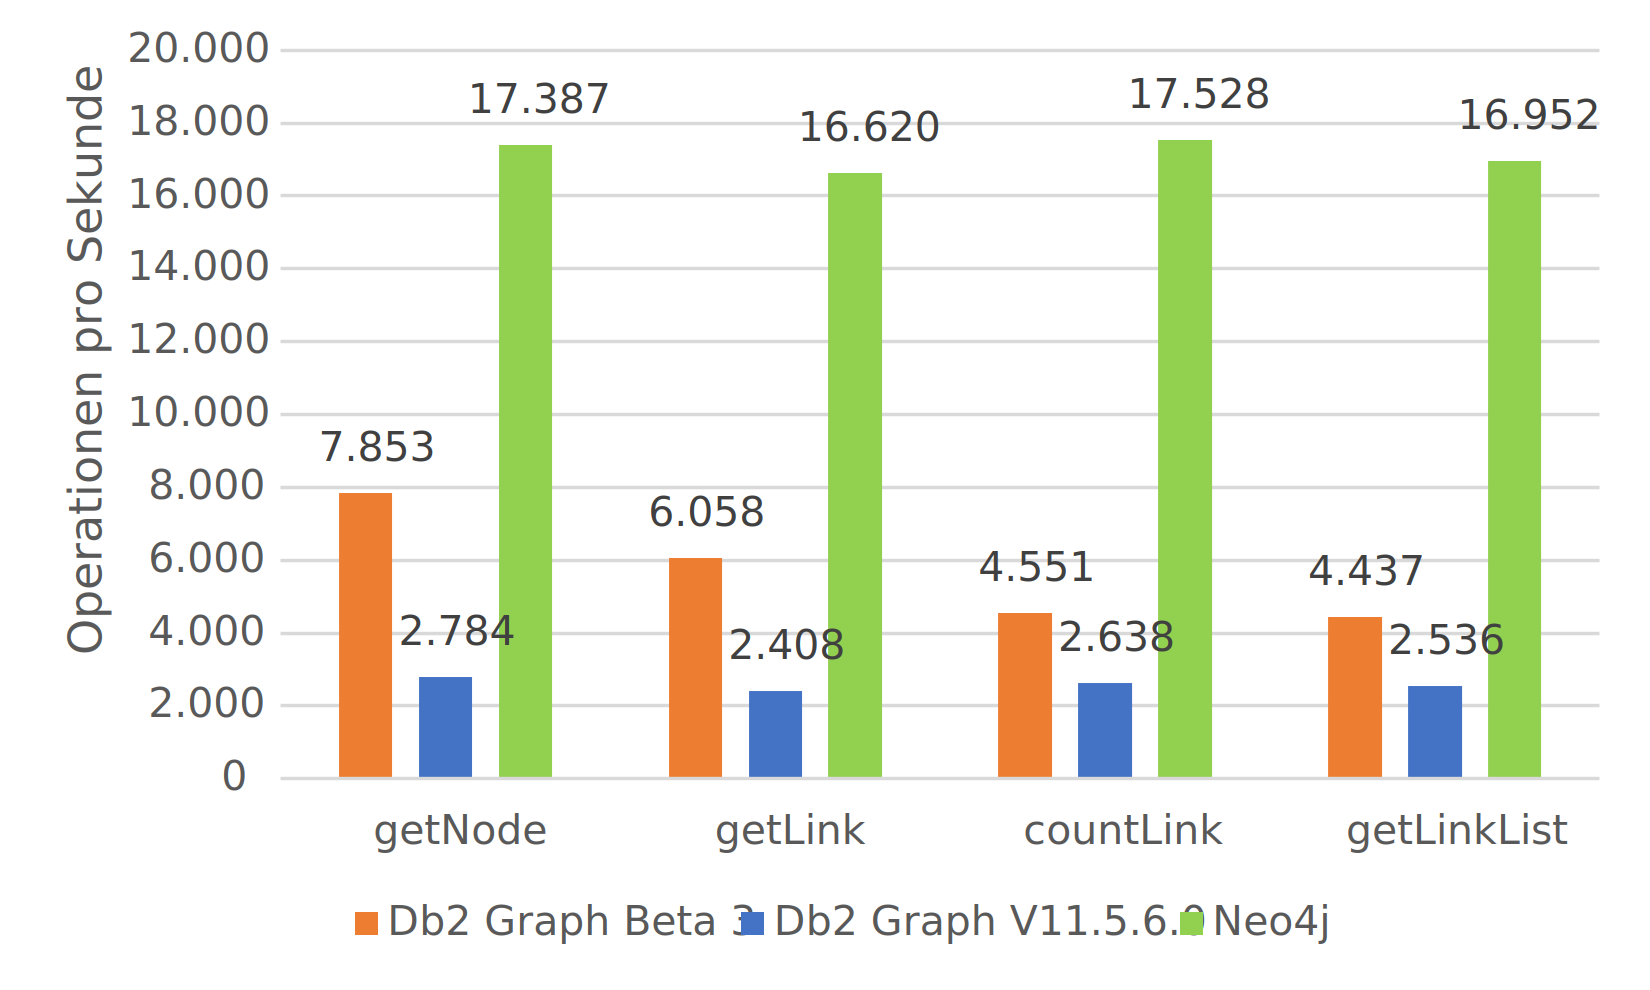
\includegraphics[width=\textwidth]{images/diagramme/linkbench_100m_const_durchsatz.pdf}
    \caption{Ergebnisse Durchsatz Linkbench-100M-Const}
    \label{fig:durchsatz:linkbench_100m_const}
\end{figure}

\section{Linkbench-10M-Real}
\label{ergebnisse:10m_real}
In diesem Abschnitt werden die Ergebnisse für die Messreihe \nameref{ergebnisse:10m_real} dargestellt und untersucht. Hierbei handelt es sich um die ersten Messergebnisse die für einen (kleinen) real-verteilten Datensatz erzielt wurden. So beinhalten die hier aufgeführten Messergebnisse sowohl Latenz- als auch Durchsatzwerte für die \texttt{getLinkList}-Operation mit jeweils verschieden hohen Ergebnismenge. Das Datenbanksystem Db2 Graph Beta 3 spielt in den Messungen hingehen keine Rolle.

\subsection{Latenz}
Bei der Analyse der Latenzwerte von Db2 Graph V11.5.6.0 (\autoref{tab:latenz_10m_real:ga} und \autoref{tab:latenz_10m_real:ga:gll}) und Neo4j (\autoref{tab:latenz_10m_real:neo4j} und \autoref{tab:latenz_10m_real:neo4j:gll}) bietet sich ein ähnlicher Anblick, wie bei den konstant-verteilten Datensätzen. Neo4j weist weitaus geringere Latenzergebnisse auf als Db2 Graph V11.5.6.0. 

Dabei fällt allerdings auf, dass die durchschnittlichen Latenzen bei Db2 Graph V11.5.6.0 vergleichbar hoch sind wie in \autoref{tab:latenz_10m_const:ga} bei der Messreihe \nameref{ergebnisse:10m_const} mit dem kleineren konstant-verteilten Datensatz. Dies ist außergewöhnlich, da sich die Datensätze nicht nur bezüglich der Verteilung, sondern auch was die Größe beziehungsweise die Kantenanzahl betrifft, erheblich unterscheiden.

\begin{table}[!h]
\centering
\resizebox{\textwidth}{!}{
\begin{tabular}{l|r|r|r|r|r|r|r}
\hline
\rowcolor[HTML]{EFEFEF} 
\multicolumn{1}{c|}{\cellcolor[HTML]{EFEFEF}\textbf{Operation}} &
\multicolumn{1}{c|}{\cellcolor[HTML]{EFEFEF}\textbf{Mean}} &
\multicolumn{1}{c|}{\cellcolor[HTML]{EFEFEF}\textbf{p25}} &
\multicolumn{1}{c|}{\cellcolor[HTML]{EFEFEF}\textbf{p50}} &
\multicolumn{1}{c|}{\cellcolor[HTML]{EFEFEF}\textbf{p75}} &
\multicolumn{1}{c|}{\cellcolor[HTML]{EFEFEF}\textbf{p95}} &
\multicolumn{1}{c|}{\cellcolor[HTML]{EFEFEF}\textbf{p99}} &
\multicolumn{1}{c}{\cellcolor[HTML]{EFEFEF}\textbf{Max.}} \\ \hline
getNode & 17,88ms & {[}4,5{]}ms & {[}13,14{]}ms & {[}29,30{]}ms & {[}42,43{]}ms & {[}49,50{]}ms & 293,64ms \\
getLink & 20,47ms & {[}6,7{]}ms & {[}14,15{]}ms & {[}33,34{]}ms & {[}49,50{]}ms & {[}57,58{]}ms & 356,93ms \\
countLink & 18,32ms & {[}5,6{]}ms & {[}12,13{]}ms & {[}30,31{]}ms & {[}44,45{]}ms & {[}51,52{]}ms & 277,05ms \\ \hline
\end{tabular}
}
\caption{Latenz Linkbench-10M-Real Db2 Graph V11.5.6.0}
\label{tab:latenz_10m_real:ga}
\end{table}    

\begin{table}[!h]
\centering
\resizebox{\textwidth}{!}{
\begin{tabular}{r|r|r|r|r|r|r|r}
\hline
\rowcolor[HTML]{EFEFEF} 
\multicolumn{1}{c|}{\cellcolor[HTML]{EFEFEF}\textbf{Mean}} &
\multicolumn{1}{c|}{\cellcolor[HTML]{EFEFEF}\textbf{p25}} &
\multicolumn{1}{c|}{\cellcolor[HTML]{EFEFEF}\textbf{p50}} &
\multicolumn{1}{c|}{\cellcolor[HTML]{EFEFEF}\textbf{p75}} &
\multicolumn{1}{c|}{\cellcolor[HTML]{EFEFEF}\textbf{p95}} &
\multicolumn{1}{c|}{\cellcolor[HTML]{EFEFEF}\textbf{p99}} &
\multicolumn{1}{c|}{\cellcolor[HTML]{EFEFEF}\textbf{Max.}} &
\multicolumn{1}{c}{\cellcolor[HTML]{EFEFEF}\textbf{Limit}} \\ \hline
19,64ms & {[}5,6{]}ms & {[}13,14{]}ms & {[}32,33{]}ms & {[}47,48{]}ms & {[}55,56{]}ms & 401,99ms & 100\\
20,12ms & {[}5,6{]}ms & {[}14,15{]}ms & {[}32,33{]}ms & {[}48,49{]}ms & {[}57,58{]}ms & 442,84ms & 1.000\\
22,37ms & {[}5,6{]}ms & {[}15,16{]}ms & {[}35,36{]}ms & {[}53,54{]}ms & {[}68,69{]}ms & 776,83ms & 10.000\\
34,00ms & {[}6,7{]}ms & {[}20,21{]}ms & {[}44,45{]}ms & {[}82,83{]}ms & {[}100,200{]}ms & 3.125,17ms & 100.000\\ \hline
\end{tabular}
}
\caption{Latenz Linkbench-10M-Real Db2 Graph V11.5.6.0 getLinkList}
\label{tab:latenz_10m_real:ga:gll}
\end{table}

\begin{table}[!h]
\centering
\resizebox{\textwidth}{!}{
\begin{tabular}{l|r|r|r|r|r|r|r}
\hline
\rowcolor[HTML]{EFEFEF} 
\multicolumn{1}{c|}{\cellcolor[HTML]{EFEFEF}\textbf{Operation}} &
\multicolumn{1}{c|}{\cellcolor[HTML]{EFEFEF}\textbf{Mean}} &
\multicolumn{1}{c|}{\cellcolor[HTML]{EFEFEF}\textbf{p25}} &
\multicolumn{1}{c|}{\cellcolor[HTML]{EFEFEF}\textbf{p50}} &
\multicolumn{1}{c|}{\cellcolor[HTML]{EFEFEF}\textbf{p75}} &
\multicolumn{1}{c|}{\cellcolor[HTML]{EFEFEF}\textbf{p95}} &
\multicolumn{1}{c|}{\cellcolor[HTML]{EFEFEF}\textbf{p99}} &
\multicolumn{1}{c}{\cellcolor[HTML]{EFEFEF}\textbf{Max.}} \\ \hline
getNode & 2,89ms & {[}2,3{]}ms & {[}2,3{]}ms & {[}3,4{]}ms & {[}3,4{]}ms & {[}5,6{]}ms & 1.073,54ms \\
getLink & 3,30ms & {[}2,3{]}ms & {[}2,3{]}ms & {[}3,4{]}ms & {[}5,6{]}ms & {[}9,10{]}ms & 2.433,82ms \\
countLink & 3,05ms & {[}2,3{]}ms & {[}2,3{]}ms & {[}3,4{]}ms & {[}4,5{]}ms & {[}8,9{]}ms & 1.381,42ms \\ \hline
\end{tabular}
}
\caption{Latenz Linkbench-10M-Real Neo4j}
\label{tab:latenz_10m_real:neo4j}
\end{table}

\begin{table}[!h]
\centering
\resizebox{\textwidth}{!}{
\begin{tabular}{l|r|r|r|r|r|r|r}
\hline
\rowcolor[HTML]{EFEFEF} 
\multicolumn{1}{c|}{\cellcolor[HTML]{EFEFEF}\textbf{Operation}} &
\multicolumn{1}{c|}{\cellcolor[HTML]{EFEFEF}\textbf{Mean}} &
\multicolumn{1}{c|}{\cellcolor[HTML]{EFEFEF}\textbf{p25}} &
\multicolumn{1}{c|}{\cellcolor[HTML]{EFEFEF}\textbf{p50}} &
\multicolumn{1}{c|}{\cellcolor[HTML]{EFEFEF}\textbf{p75}} &
\multicolumn{1}{c|}{\cellcolor[HTML]{EFEFEF}\textbf{p95}} &
\multicolumn{1}{c|}{\cellcolor[HTML]{EFEFEF}\textbf{p99}} &
\multicolumn{1}{c}{\cellcolor[HTML]{EFEFEF}\textbf{Max.}} \\ \hline
getLinkList & 3,08ms & {[}2,3{]}ms & {[}2,3{]}ms & {[}3,4{]}ms & {[}4,5{]}ms & {[}8,9{]}ms & 1.021,83ms \\
getLinkList & 3,42ms & {[}2,3{]}ms & {[}2,3{]}ms & {[}3,4{]}ms & {[}6,7{]}ms & {[}11,12{]}ms & 982,84ms \\
getLinkList & 4,38ms & {[}2,3{]}ms & {[}3,4{]}ms & {[}4,5{]}ms & {[}8,9{]}ms & {[}16,17{]}ms & 1.041,73ms \\
getLinkList & 5,46ms & {[}2,3{]}ms & {[}2,3{]}ms & {[}4,5{]}ms & {[}8,9{]}ms & {[}21,22{]}ms & 1.855,68ms \\ \hline
\end{tabular}
}
\caption{Latenz Linkbench-10M-Real Neo4j getLinkList}
\label{tab:latenz_10m_real:neo4j:gll}
\end{table}

In Bezug zu den Latenzwerten für die \texttt{getLinkList}-Operation mit jeweils unterschiedlichen Grenzen für die Ergebnismenge fällt auf, dass die ursprünglichen Durchschnittslatenzen von Db2 Graph V11.5.6.0 und Neo4j zwischen den Messungen mit einer maximalen Ergebnismenge von 100 und 100.000 nahezu verdoppeln.

\subsection{Durchsatz}
Die im Kontext dieser Messreihe ermittelten Durchsatzwerte (\autoref{fig:durchsatz:linkbench_10m_real} und \autoref{fig:durchsatz:linkbench_10m_real:rl}) bestätigen die bereits bei den Latenzen entdeckten Phänomene. So weist Neo4j durch den höheren Durchsatz bei allen gebenchmarkten Operationen eine bessere Performance als Db2 Graph V11.5.6.0 auf. 

Des Weiteren scheinen auch hier die Werte für Db2 Graph V11.5.6.0 in \autoref{fig:durchsatz:linkbench_10m_real} überraschenderweise denen aus \autoref{fig:durchsatz:linkbench_10m_const} zu ähneln, trotz eines unterschiedlichen Datensatzes.

\begin{figure}[!ht]
    \centering
    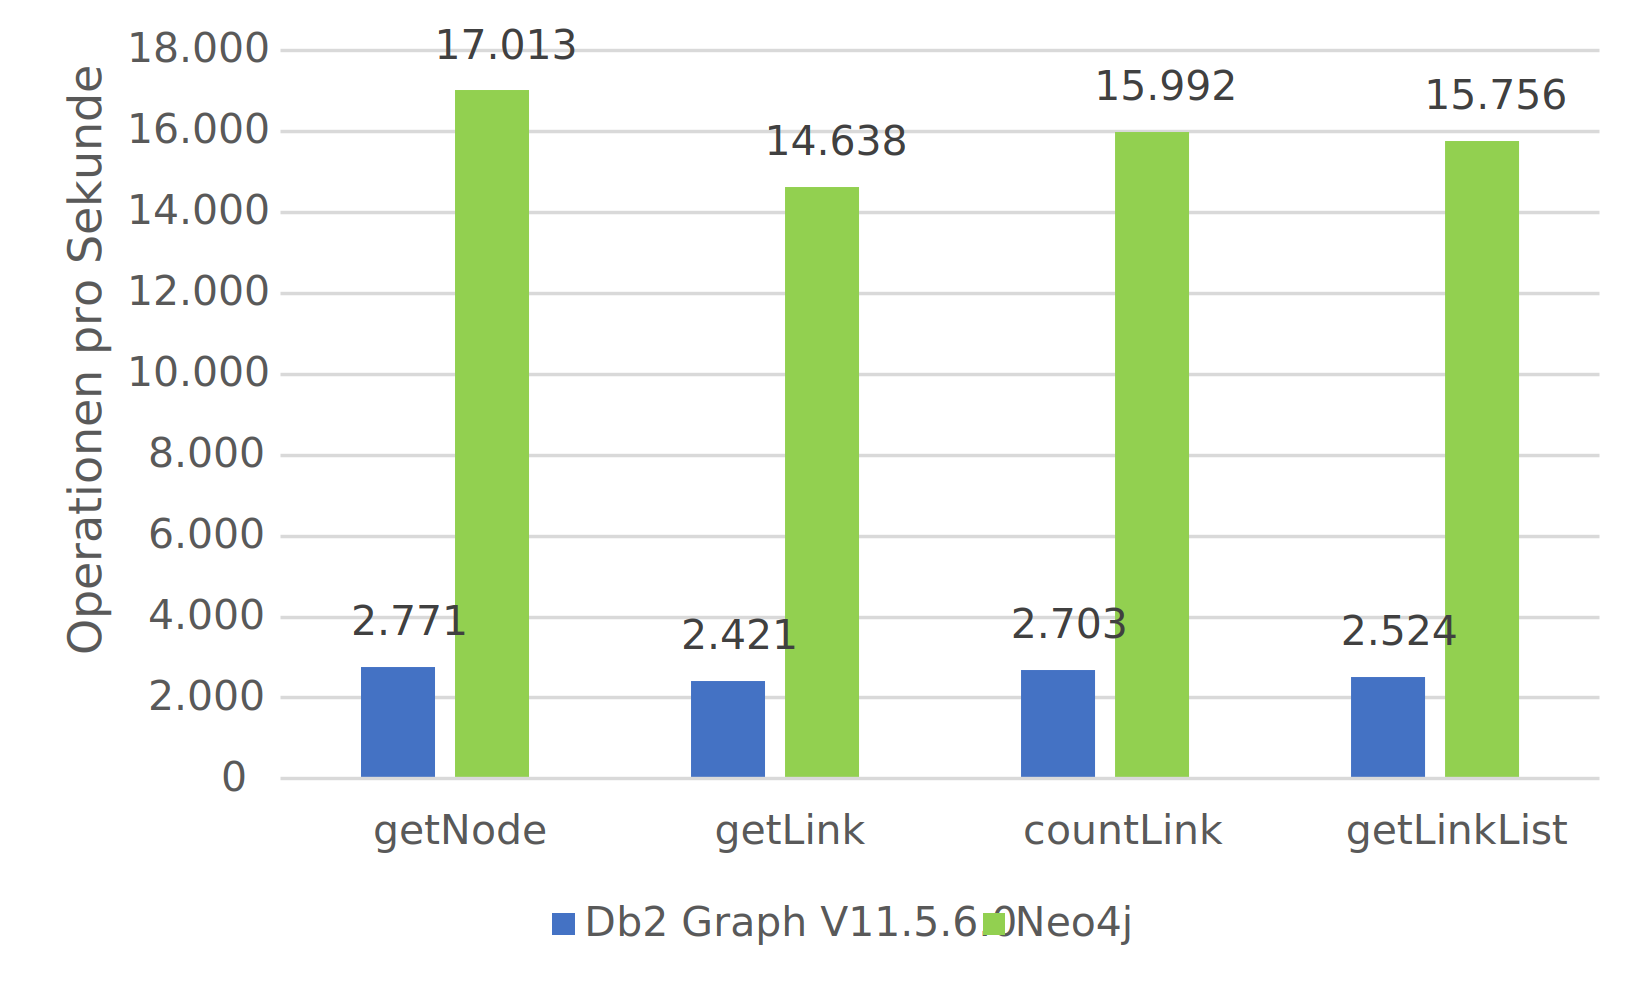
\includegraphics[width=\textwidth]{images/diagramme/linkbench_10m_real_durchsatz.pdf}
    \caption{Ergebnisse Durchsatz Linkbench-10M-Real}
    \label{fig:durchsatz:linkbench_10m_real}
    \vspace{1em}
    \textit{Die bei getLinkList abgebildeten Werte repräsentieren die Ergebnisse, die mit einer Begrenzung der Ergebnismenge auf maximal 100 Elemente erzielt wurden.}
\end{figure}

\begin{figure}[!ht]
    \centering
    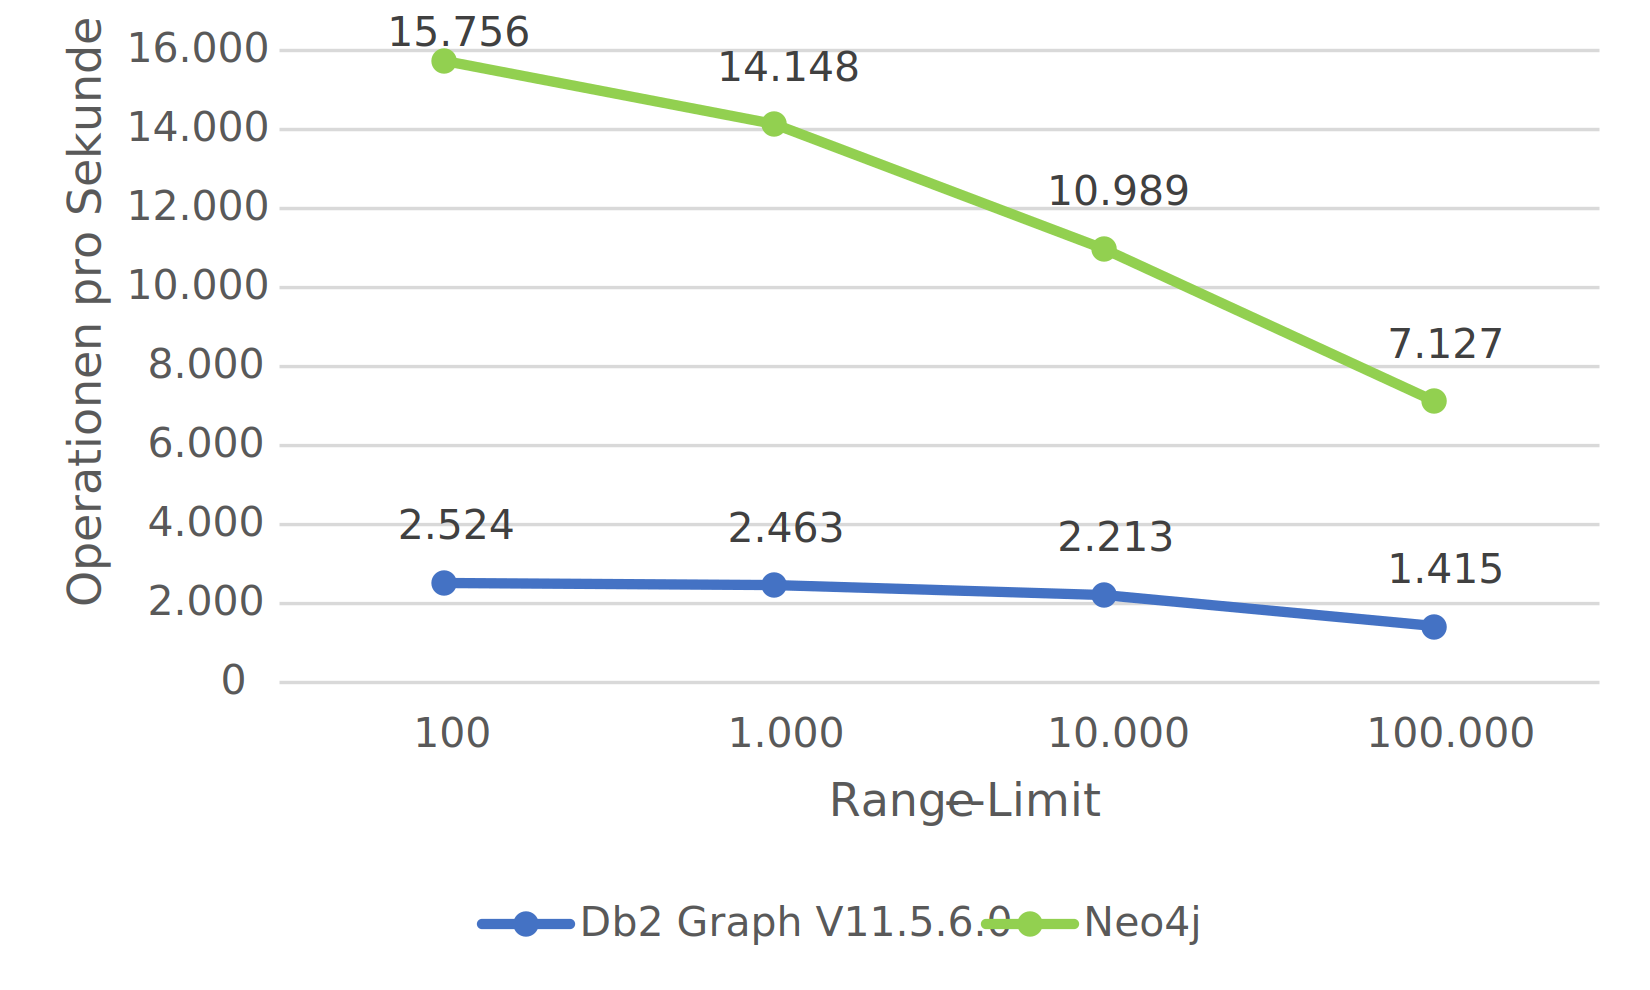
\includegraphics[width=\textwidth]{images/diagramme/limit_absolute_durchsatz_real_10m.pdf}
    \caption{Ergebnisse Durchsatz Linkbench-10M-Real getLinkList}
    \label{fig:durchsatz:linkbench_10m_real:rl}
\end{figure}

Analog zu den Latenzwerten halbieren sich auch die Durchsatzergebnisse der \texttt{getLinkList}-Operation zwischen den Messungen mit einem Range-Limit von 100 und 100.000 bei beiden Datenbanksystemen.

\section{Linkbench-100M-Real}
\label{ergebnisse:100m_real}
Im Rahmen dieses Abschnitts werden die Latenz- und Durchsatzergebnisse für Db2 Graph V11.5.6.0 und Neo4j aufgeführt. Alle Messungen deren Ergebnisse hier zur Schau gestellt werden, wurden auf Basis eines größeren real-verteilten Datensatzes erzielt. So umfasst der Datensatz dieser Messreihe (\nameref{ergebnisse:100m_real}) die zehnfache Anzahl an Knoten und Kanten wie der Datensatz der Messreihe \nameref{ergebnisse:10m_real}. Im Kontext dieser Ergebnisse spielt Db2 Graph Beta 3 wie bereits bei \nameref{ergebnisse:10m_real} keine Rolle. Darüber hinaus existieren  ebenfalls mehrere Messergebnisse für die \texttt{getLinkList}-Operation mit einer variierenden Beschränkung der Ergebnismenge.

\subsection{Latenz}
Bei der Untersuchung der Latenzwerte von Db2 Graph V11.5.6.0 (\autoref{tab:latenz_100m_real:ga} und \autoref{tab:latenz_100m_real:ga:gll}) und Neo4j (\autoref{tab:latenz_100m_real:neo4j} und \autoref{tab:latenz_100m_real:neo4j:gll}) fällt auf, dass Neo4j wieder deutlich niedrigere Durchschnittslatenzen aufweist als Db2 Graph V11.5.6.0. 

Die Messergebnisse für die Latenzen beider Datenbanksysteme ähneln dabei denen des kleineren real-verteilten Datensatzes aus \nameref{ergebnisse:10m_real}. Dieses Verhalten könnte sich wie bereits bei den konstant-verteilten Datensätzen basierten Messreihen damit erklären, dass Db2 und Neo4j beiden um einen Bufferpool und Page-Cache verfügen, in alle Datensätze vollständig geladen werden können, egal ob Linkbench-10M oder Linkbench-100M.

Des Weiteren fällt auch beim Vergleich der Werte von \autoref{tab:latenz_100m_const:ga} mit \autoref{tab:latenz_100m_real:ga} und \autoref{tab:latenz_100m_real:ga:gll} auf, dass sich die durchschnittlichen Latenzen überraschend ähneln, obwohl sich die Größe und Verteilung der Datensätze bei \nameref{ergebnisse:100m_const} und dieser Messreihe erheblich unterscheiden.

Bei der Analyse der durchschnittlichen Latenzen der \texttt{getLinkList}-Operationen mit variierender Ergebnismenge kann hierbei identifiziert werden, dass die Db2 Graph V11.5.6.0  (\autoref{tab:latenz_10m_real:ga}) und Neo4j Werte beide bei der steigenden Beschränkung der Ergebnismenge deutlich erhöhen. Bei Neo4j verdoppelt sich hierbei die durchschnittliche Latenz sogar, während dies bei Db2 Graph V11.5.6.0 nicht der Fall ist.

\begin{table}[!ht]
\centering
\resizebox{\textwidth}{!}{
\begin{tabular}{l|r|r|r|r|r|r|r}
\hline
\rowcolor[HTML]{EFEFEF} 
\multicolumn{1}{c|}{\cellcolor[HTML]{EFEFEF}\textbf{Operation}} &
\multicolumn{1}{c|}{\cellcolor[HTML]{EFEFEF}\textbf{Mean}} &
\multicolumn{1}{c|}{\cellcolor[HTML]{EFEFEF}\textbf{p25}} &
\multicolumn{1}{c|}{\cellcolor[HTML]{EFEFEF}\textbf{p50}} &
\multicolumn{1}{c|}{\cellcolor[HTML]{EFEFEF}\textbf{p75}} &
\multicolumn{1}{c|}{\cellcolor[HTML]{EFEFEF}\textbf{p95}} &
\multicolumn{1}{c|}{\cellcolor[HTML]{EFEFEF}\textbf{p99}} &
\multicolumn{1}{c}{\cellcolor[HTML]{EFEFEF}\textbf{Max.}} \\ \hline
getNode & 17,91ms & {[}5,6{]}ms & {[}13,14{]}ms & {[}29,30{]}ms & {[}42,43{]}ms & {[}49,50{]}ms & 520,53ms \\
getLink & 20,91ms & {[}7,8{]}ms & {[}14,15{]}ms & {[}33,34{]}ms & {[}49,50{]}ms & {[}57,58{]}ms & 811,52ms \\
countLink & 18,88ms & {[}5,6{]}ms & {[}13,14{]}ms & {[}30,31{]}ms & {[}45,46{]}ms & {[}52,53{]}ms & 661,18ms \\ \hline
\end{tabular}
}
\caption{Latenz Linkbench-100-Real Db2 Graph V11.5.6.0}
\label{tab:latenz_100m_real:ga}
\end{table}

\begin{table}[!ht]
\centering
\resizebox{\textwidth}{!}{
\begin{tabular}{r|r|r|r|r|r|r|r}
\hline
\rowcolor[HTML]{EFEFEF} 
\multicolumn{1}{c|}{\cellcolor[HTML]{EFEFEF}\textbf{Mean}} &
\multicolumn{1}{c|}{\cellcolor[HTML]{EFEFEF}\textbf{p25}} &
\multicolumn{1}{c|}{\cellcolor[HTML]{EFEFEF}\textbf{p50}} &
\multicolumn{1}{c|}{\cellcolor[HTML]{EFEFEF}\textbf{p75}} &
\multicolumn{1}{c|}{\cellcolor[HTML]{EFEFEF}\textbf{p95}} &
\multicolumn{1}{c|}{\cellcolor[HTML]{EFEFEF}\textbf{p99}} &
\multicolumn{1}{c|}{\cellcolor[HTML]{EFEFEF}\textbf{Max.}} &
\multicolumn{1}{c}{\cellcolor[HTML]{EFEFEF}\textbf{Limit}} \\ \hline
20,06ms & {[}6,7{]}ms & {[}14,15{]}ms & {[}32,33{]}ms & {[}47,48{]}ms & {[}54,55{]}ms & 502,66ms & 100\\
20,78ms & {[}6,7{]}ms & {[}14,15{]}ms & {[}33,34{]}ms & {[}49,50{]}ms & {[}58,59{]}ms & 2.003,24ms & 1.000\\
22,56ms & {[}6,7{]}ms & {[}15,16{]}ms & {[}35,36{]}ms & {[}53,54{]}ms & {[}67,68{]}ms & 2.553,64ms & 10.000\\
36,62ms & {[}7,8{]}ms & {[}21,22{]}ms & {[}46,47{]}ms & {[}89,90{]}ms & {[}100,200{]}ms & 4.351,98ms & 100.000\\ \hline
\end{tabular}
}
\caption{Latenz Linkbench-100M-Real Db2 Graph V11.5.6.0 getLinkList}
\label{tab:latenz_100m_real:ga:gll}
\end{table}

\begin{table}[!ht]
\centering
\resizebox{\textwidth}{!}{
\begin{tabular}{l|r|r|r|r|r|r|r}
\hline
\rowcolor[HTML]{EFEFEF} 
\multicolumn{1}{c|}{\cellcolor[HTML]{EFEFEF}\textbf{Operation}} &
\multicolumn{1}{c|}{\cellcolor[HTML]{EFEFEF}\textbf{Mean}} &
\multicolumn{1}{c|}{\cellcolor[HTML]{EFEFEF}\textbf{p25}} &
\multicolumn{1}{c|}{\cellcolor[HTML]{EFEFEF}\textbf{p50}} &
\multicolumn{1}{c|}{\cellcolor[HTML]{EFEFEF}\textbf{p75}} &
\multicolumn{1}{c|}{\cellcolor[HTML]{EFEFEF}\textbf{p95}} &
\multicolumn{1}{c|}{\cellcolor[HTML]{EFEFEF}\textbf{p99}} &
\multicolumn{1}{c}{\cellcolor[HTML]{EFEFEF}\textbf{Max.}} \\ \hline
getNode & 2,86ms & {[}2,3{]}ms & {[}2,3{]}ms & {[}3,4{]}ms & {[}3,4{]}ms & {[}5,6{]}ms & 786,65ms \\
getLink & 3,26ms & {[}2,3{]}ms & {[}2,3{]}ms & {[}3,4{]}ms & {[}5,6{]}ms & {[}9,10{]}ms & 2.387,52ms \\
countLink & 3,05ms & {[}2,3{]}ms & {[}2,3{]}ms & {[}3,4{]}ms & {[}4,5{]}ms & {[}8,9{]}ms & 1.510,54ms \\ \hline
\end{tabular}
}
\caption{Latenz Linkbench-100M-Real Neo4j}
\label{tab:latenz_100m_real:neo4j}
\end{table}

\begin{table}[!ht]
\centering
\resizebox{\textwidth}{!}{
\begin{tabular}{r|r|r|r|r|r|r|r}
\hline
\rowcolor[HTML]{EFEFEF} 
\multicolumn{1}{c|}{\cellcolor[HTML]{EFEFEF}\textbf{Mean}} &
\multicolumn{1}{c|}{\cellcolor[HTML]{EFEFEF}\textbf{p25}} &
\multicolumn{1}{c|}{\cellcolor[HTML]{EFEFEF}\textbf{p50}} &
\multicolumn{1}{c|}{\cellcolor[HTML]{EFEFEF}\textbf{p75}} &
\multicolumn{1}{c|}{\cellcolor[HTML]{EFEFEF}\textbf{p95}} &
\multicolumn{1}{c|}{\cellcolor[HTML]{EFEFEF}\textbf{p99}} &
\multicolumn{1}{c|}{\cellcolor[HTML]{EFEFEF}\textbf{Max.}} &
\multicolumn{1}{c}{\cellcolor[HTML]{EFEFEF}\textbf{Limit}} \\ \hline
3,09ms & {[}2,3{]}ms & {[}2,3{]}ms & {[}3,4{]}ms & {[}4,5{]}ms & {[}8,9{]}ms & 927,23ms & 100\\
3,39ms & {[}2,3{]}ms & {[}2,3{]}ms & {[}3,4{]}ms & {[}6,7{]}ms & {[}11,12{]}ms & 1.056,44ms & 1.000\\
4,37ms & {[}2,3{]}ms & {[}3,4{]}ms & {[}4,5{]}ms & {[}8,9{]}ms & {[}16,17{]}ms & 1.157,71ms & 10.000\\
6,53ms & {[}2,3{]}ms & {[}3,4{]}ms & {[}4,5{]}ms & {[}10,11{]}ms & {[}29,30{]}ms & 2.037,55ms & 100.000\\ \hline
\end{tabular}
}
\caption{Latenz Linkbench-100M-Real Neo4j getLinkList}
\label{tab:latenz_100m_real:neo4j:gll}
\end{table}

\subsection{Durchsatz}
Die in \autoref{fig:durchsatz:linkbench_100m_real} und \autoref{fig:durchsatz:linkbench_100m_real:rl} aufgeführten Durchsatzwerte verifizieren die Beobachtungen, die bereits bei den Latenzen gemacht wurden. So weist Neo4j wieder einen höheren Durchsatz als Db2 Graph V11.5.6.0 auf.

Darüber hinaus ähneln auch die im Rahmen dieser Messreihe erzielten Durchsatzergebnisse (\autoref{fig:durchsatz:linkbench_100m_real}) denen des kleineren real-verteilten Datensatzes (\autoref{fig:durchsatz:linkbench_10m_real}). 

Auch scheinen die Durchsatzergebnisse für Db2 Graph V11.5.6.0 hier (\autoref{fig:durchsatz:linkbench_100m_real}) und in \nameref{fig:durchsatz:linkbench_100m_const} (\autoref{fig:durchsatz:linkbench_100m_const}) überraschend nah bei einander zu liegen, obwohl sich die Datensätze bei den Messungen signifikant in ihrer Größe und Verteilung unterscheiden. 

Des Weiteren halbiert sich auch hier ungefähr der Durchsatz beim Anstieg des Range-Limits von 100 auf 100.000, passend zur Verdoppelung bei den Latenzwerten.

\begin{figure}[!ht]
    \centering
    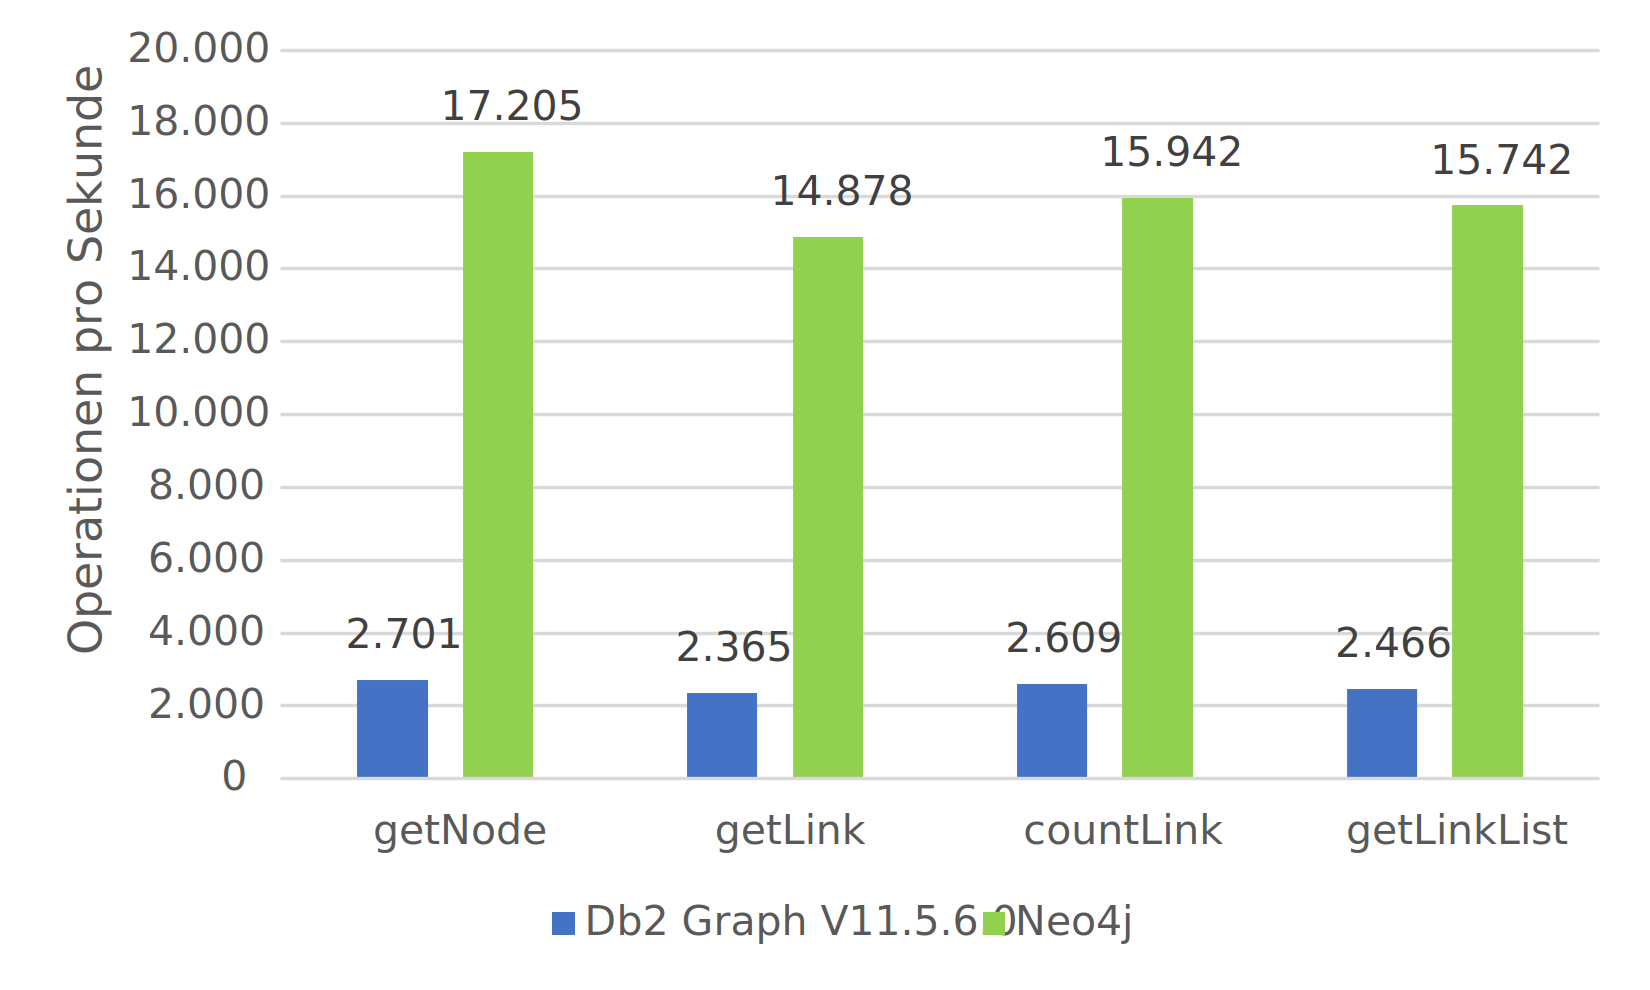
\includegraphics[width=\textwidth]{images/diagramme/linkbench_100m_real_durchsatz.pdf}
    \caption{Ergebnisse Durchsatz Linkbench-10M-Real}
    \label{fig:durchsatz:linkbench_100m_real}
    \vspace{1em}
    \textit{Die bei getLinkList abgebildeten Werte repräsentieren die Ergebnisse, die mit einer Begrenzung der Ergebnismenge auf maximal 100 Elemente erzielt wurden.}
\end{figure}

\begin{figure}[!ht]
    \centering
    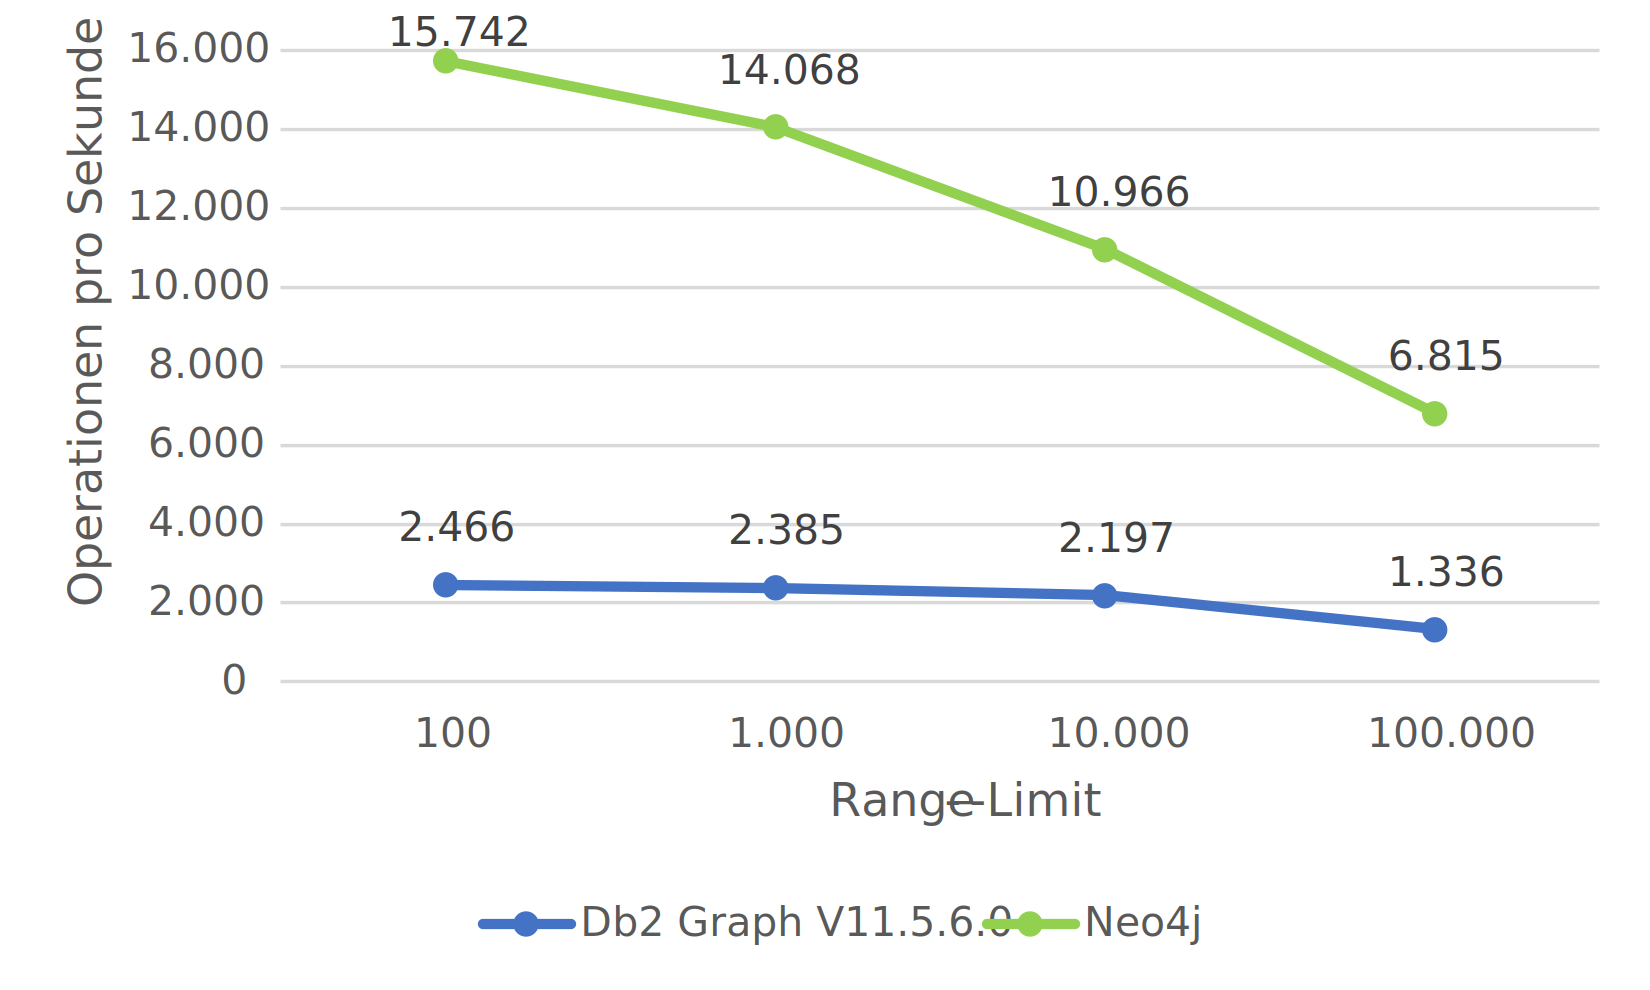
\includegraphics[width=\textwidth]{images/diagramme/limit_absolute_durchsatz_real_100m.pdf}
    \caption{Ergebnisse Durchsatz Linkbench-10M-Real getLinkList}
    \label{fig:durchsatz:linkbench_100m_real:rl}
\end{figure}

\section{Auswertung}
Im Rahmen dieses Abschnitts werden die verschiedenen Phänomene und Aspekte, die bereits bei der Betrachtung und Interpretation der Ergebnisse der Messreihe angesprochen werden, nochmals aufgegriffen und isoliert betrachtet. Dabei werden hauptsächlich die Durchsatzergebnisse herangezogen, da der Fokus bei der Besprechung der Messreihen in \autoref{ergebnisse} bereits hauptsächlich auf die Latenzwerte gelegt wird. So werden auch die Durchsatzangaben nochmals genauer aufgegriffen. Außerdem wird in \autoref{ergebnisse} bereits die Beobachtung gemacht, dass Latenz- und Durchsatzwerte beide ähnliche Ergebnisse aufweisen, bei welcher Messung der Durchsatz hoch ist bei der ist auch die Latenz niedrig und umgekehrt.

\subsection{Einordnung der Performance}
Bei der Beurteilung der Performance der Datenbanksysteme handelt es sich bei den im Rahmen der Arbeit erzielten Messergebnissen um eine einfache Aufgabe. So weist bei jeder Messreihe Neo4j den niedrigsten Latenz- und Durchsatzwert auf, gefolgt von Db2 Graph Beta 3 -- sollte es Teil der Messreihe sein -- und Db2 Graph V11.5.6.0. 

Bei der Betrachtung der in der Messreihe beschriebenen Ergebnisse fällt zugleich auf, dass es sich hierbei nicht um einen kleinen Unterschied zwischen den jeweiligen Datenbanksystemen handelt. So scheinen sich die Datenbanksysteme sowohl bei der durchschnittlichen Latenz als auch beim Durchsatz um einen ähnlichen Faktor zu unterscheiden. Um die Datenbanksysteme bezüglich ihrer Performance einordnen zu können, wäre ein solcher Performance-Faktor von großen 

Um eine dementsprechende Kennzahl zur Einordnung der Datenbanksysteme bezüglich ihrer Performance bereitstellen zu können, wird daher ein gemeinsamer Durchschnittswert für den Durchsatz der Operationen:
\begin{itemize}
    \item \texttt{getNode}
    \item \texttt{getLink}
    \item \texttt{countLink} und 
    \item \texttt{getLinkList} (Range-Limit 100) ermittelt.
\end{itemize}
Der gemeinsame Durchschnittswert für den Durchsatz wird dabei einmal für jedes Datenbanksystem im Kontext einer Messreihe ermittelt. Anschließend wird der niedrigste Wert einer Messreihe herangezogen -- immer Db2 Graph V11.5.6.0 -- und als Faktor eins festgelegt. Im nächsten Schritt werden basierend auf diesem Faktor eins und seinem Durchschnittswert die jeweiligen Faktoren für Neo4j und gegebenenfalls Db2 Graph Beta 3 errechnet. Die dabei erhaltenen Performance-Faktoren -- basierend auf dem Durchsatz -- werden für die Messreihen mit einem konstant-verteilten Datensatz in \autoref{fig:faktor:durchsatz:const} dargelegt, während die mit real-verteilten Datensätzen in \autoref{fig:faktor:durchsatz:real} abgebildet werden.

\begin{figure}[!ht]
    \centering
    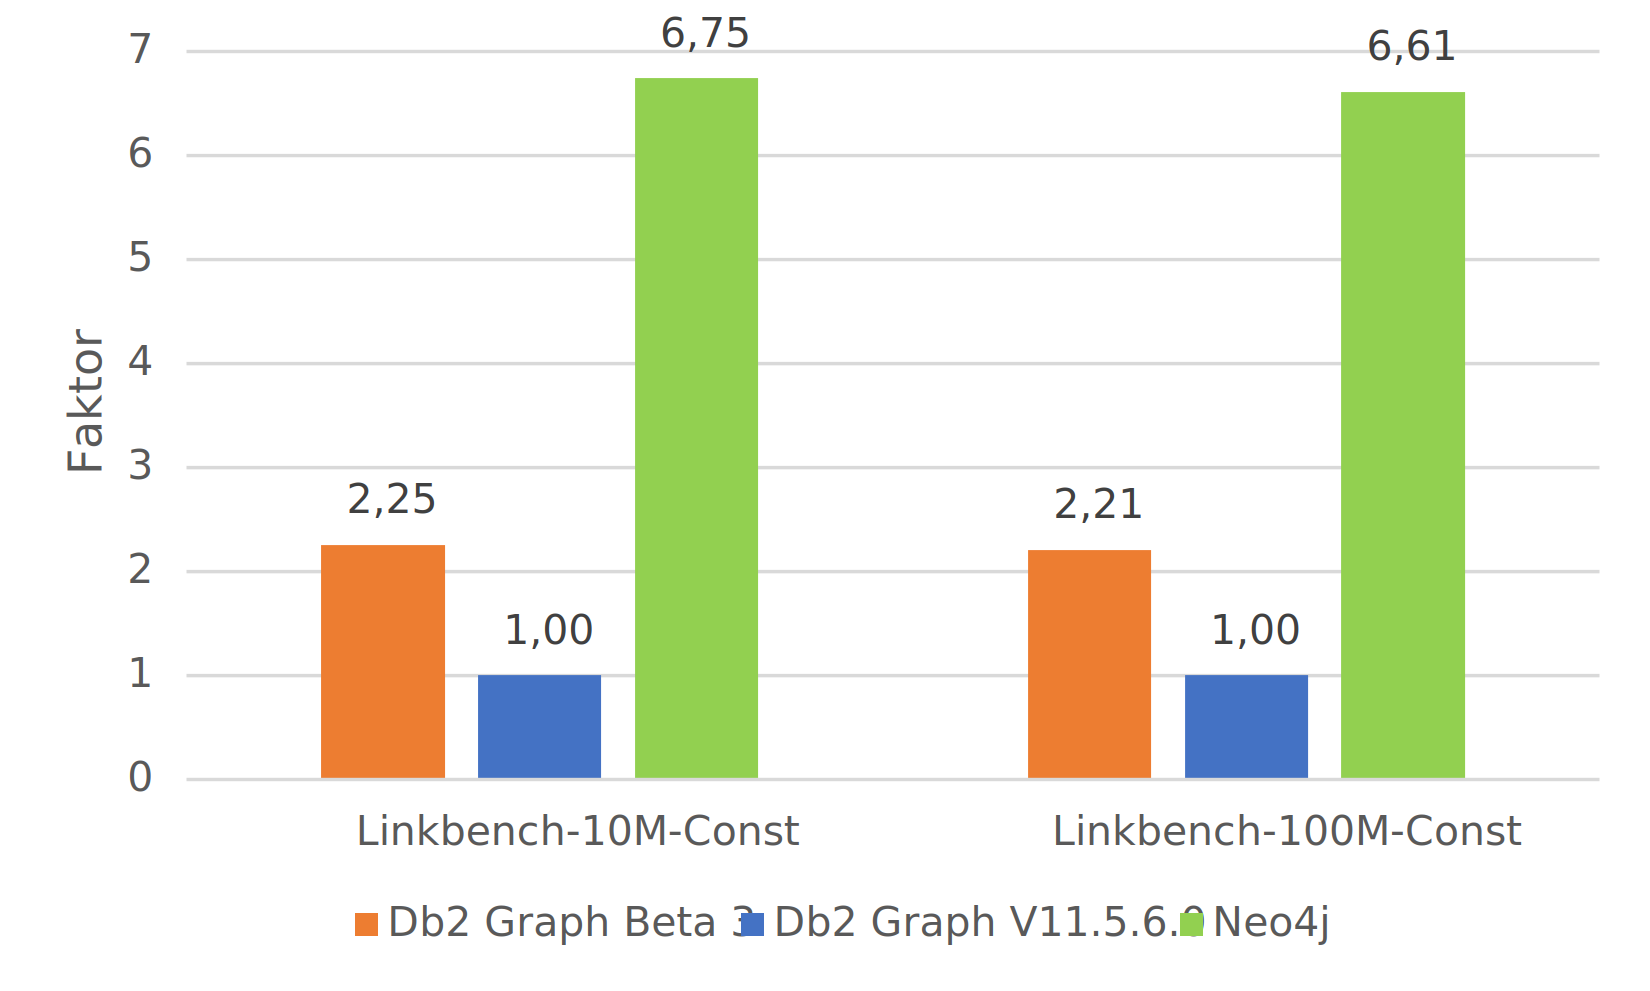
\includegraphics[width=\textwidth]{images/diagramme/faktor_durchschittlicher_durchsatz_const.pdf}
    \caption{Performance-Faktor bei Messreihen mit konstant-verteilten Datensätzen}
    \label{fig:faktor:durchsatz:const}
\end{figure}

\begin{figure}[!ht]
    \centering
    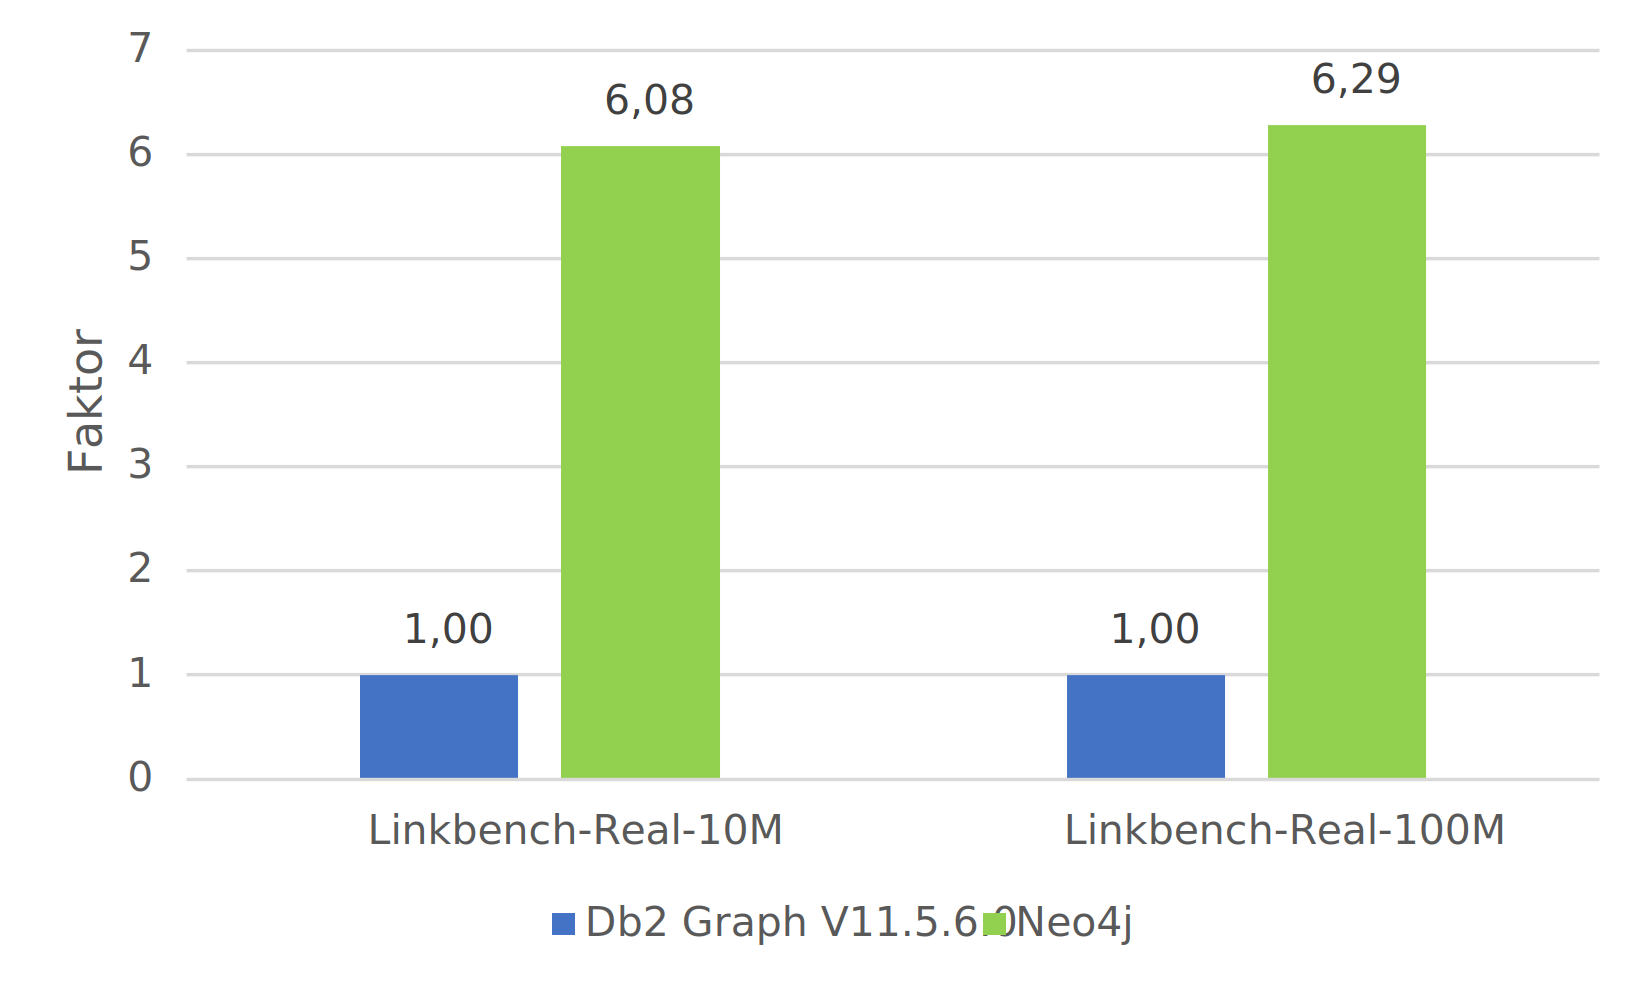
\includegraphics[width=\textwidth]{images/diagramme/faktor_durchschittlicher_durchsatz_real.pdf}
    \caption{Performance-Faktor bei Messreihen mit real-verteilten Datensätzen}
    \label{fig:faktor:durchsatz:real}
\end{figure}

Bei der Analyse der in \autoref{fig:faktor:durchsatz:const} und \autoref{fig:faktor:durchsatz:real} dargestellten Faktoren fällt auf, dass Neo4j immer 6- bis 7-Mal so viele Operationen pro Sekunde bearbeitet wie Db2 Graph bei den jeweiligen Messreihen, was einen gewaltigen Performance-Unterschied zwischen Db2 Graph V11.5.6.0 offenbart. Der Performance-Unterschied zwischen Db2 Graph Beta 3 und Neo4j um ein zwei- bis dreifaches bei den Faktoren in \autoref{fig:faktor:durchsatz:const} ist hier etwas geringer.

So war anfänglich nicht davon auszugehen das Db2 Graph als Grapherweiterung in Kombination mit Db2 Neo4j als natives Graphdatenbanksystem übertrifft. Schließlich verursacht die Kommunikation zwischen Db2 Graph und Db2, die für die Beantwortung einer Anfrage nötig ist, einen Aufwand den Neo4j nicht betreiben muss. Einen Performance-Unterschied um mindestens den Faktor 6 galt es jedoch nicht zu erwarten. 

Eine interessante Gegebenheit, die in der \autoref{fig:faktor:durchsatz:const} beobachtet werden, kann stellt der Fakt dar, dass Db2 Graph Beta 3 als ältere Version von Db2 Graph 2 bis 2,5 Mal mehr Operationen pro Sekunde bewältigen kann, als Db2 Graph V11.5.6.0 (der erste GA Release). Zu Beginn wäre hier eigentlich die Vermutung nahe gelegen, dass V11.5.6.0 als neuere Version, die über mehr Optimierungstechniken verfügt als Beta 3, eine höhere Performance aufweist. Dies scheint allerdings nicht der Fall zu sein. 

Dabei gilt es hingegen zu beachten, dass Db2 Graph Beta 3 aufgrund der höheren Performance bei den Messreihen mit konstant-verteilten Datensätzen nicht als allgemein performantere Version von Db2 Graph einzustufen ist. Schließlich spielt sie bei den Messreihen mit real-verteilten Datensätzen keine Rolle, da sie für den Einsatz dort aufgrund fehlender Optimierungstechniken derart ungeeignet war, dass das Erzielen von Ergebnissen im Rahmen des üblichen Zeitraums nicht möglich war.

\subsection{Umgang mit Ergebnismengen}
Bei der Untersuchung der Ergebnismenge bei den Messreihen mit real-verteilten Datensätzen wird bereits in \autoref{ergebnisse:10m_real} und \autoref{ergebnisse:100m_real} ein kurzer Überblick über das jeweilige Verhalten bezüglich beim Durchsatzes gegeben. Wie große der verhältnismäßige Einbruch des Durchsatzes und entsprechend auch der Performance, bei einer variierenden oberen Grenze für die Anzahl an Elementen in einer Ergebnismenge ist, lässt sich an den Abbildungen, die absolute Zahlen präsentieren, nicht ablesen. Schließlich bewegen sich die Datenbanksysteme mit beispielsweise 15.742 und 2.466 Operationen pro Sekunde in \autoref{ergebnisse:10m_real} in anderen Größenordnung, werden aber in derselben Grafik abgebildet. 

Um nun der Frage auf den Grund zugehen: \textit{Welches Datenbanksystem bei einem steigenden Range-Limit den verhältnismäßig größeren Performance-Einbruch aufweist?}, wird in \autoref{fig:einbruch:durchsatz:10m} und \autoref{fig:einbruch:durchsatz:100m} dargestellt, wie viele Prozent des Durchsatzes bei einem steigenden Range-Limit noch erreicht werden können. Der Wert für \texttt{getLinkList} mit einem Range-Limit von 100 repräsentiert dabei jeweils 100 \% des Durchsatzes von Neo4j oder Db2 Graph. So sinkt beispielsweise der Durchsatz bei Neo4j in \autoref{fig:einbruch:durchsatz:10m} bei einem Range-Limit von 10.000 auf lediglich 69,74 \% des bei einem Range-Limit von 100 erzielten Durchsatzes. 

Bei der Betrachtung des Kurvenverlaufs in \autoref{fig:einbruch:durchsatz:10m} und \autoref{fig:einbruch:durchsatz:100m} fällt auf das der Durchsatz bei Neo4j eher linear aussieht, während Db2 Graph bei einem Range-Limit von 10.000 jeweils einen Knick aufweist. 

Des Weiteren ist erkennbar, dass der Performance-Einbruch bei Db2 Graph V11.5.6.0 bei einem steigenden Range-Limit immer geringer zu sein scheint, als bei Neo4j. So weist V11.5.6.0 bei einem Range-Limit von 100.000 noch 54,18 \% des Durchsatzes auf den es bei einem Range-Limit von 100 erreicht hat. Neo4j hingegen erlangt bei 100.000 lediglich 43,29 \% des Durchsatzes den es erreicht hat, als die obere Grenze für die Ergebnismenge auf 100 Elemente begrenzt war. 

So beträgt der Unterschied zwischen Db2 Graph und Neo4j bei einem Range-Limit von 100.000 ca. 11 \% zueinander in \autoref{fig:einbruch:durchsatz:10m}, während es bei 10.000 sogar ca. 18 \% sind. Bei einem Range-Limit von 1.000 sind es jedoch lediglich ca. 8 \% Unterschied zueinander. Wobei es bei hier anzumerken gilt, dass Db2 Graph mit 97,58 \% ein außergewöhnlich hohes Ergebnis erreicht. Die in \autoref{fig:einbruch:durchsatz:100m} dargestellten Werte bestätigen dabei grob die Beobachtungen aus \autoref{fig:einbruch:durchsatz:10m}. So weichen die Werte in den beiden Abbildungen (\autoref{fig:einbruch:durchsatz:10m} und \autoref{fig:einbruch:durchsatz:100m}) höchstens um bis zu 2 \% voneinander ab. 

\begin{figure}[!ht]
    \centering
    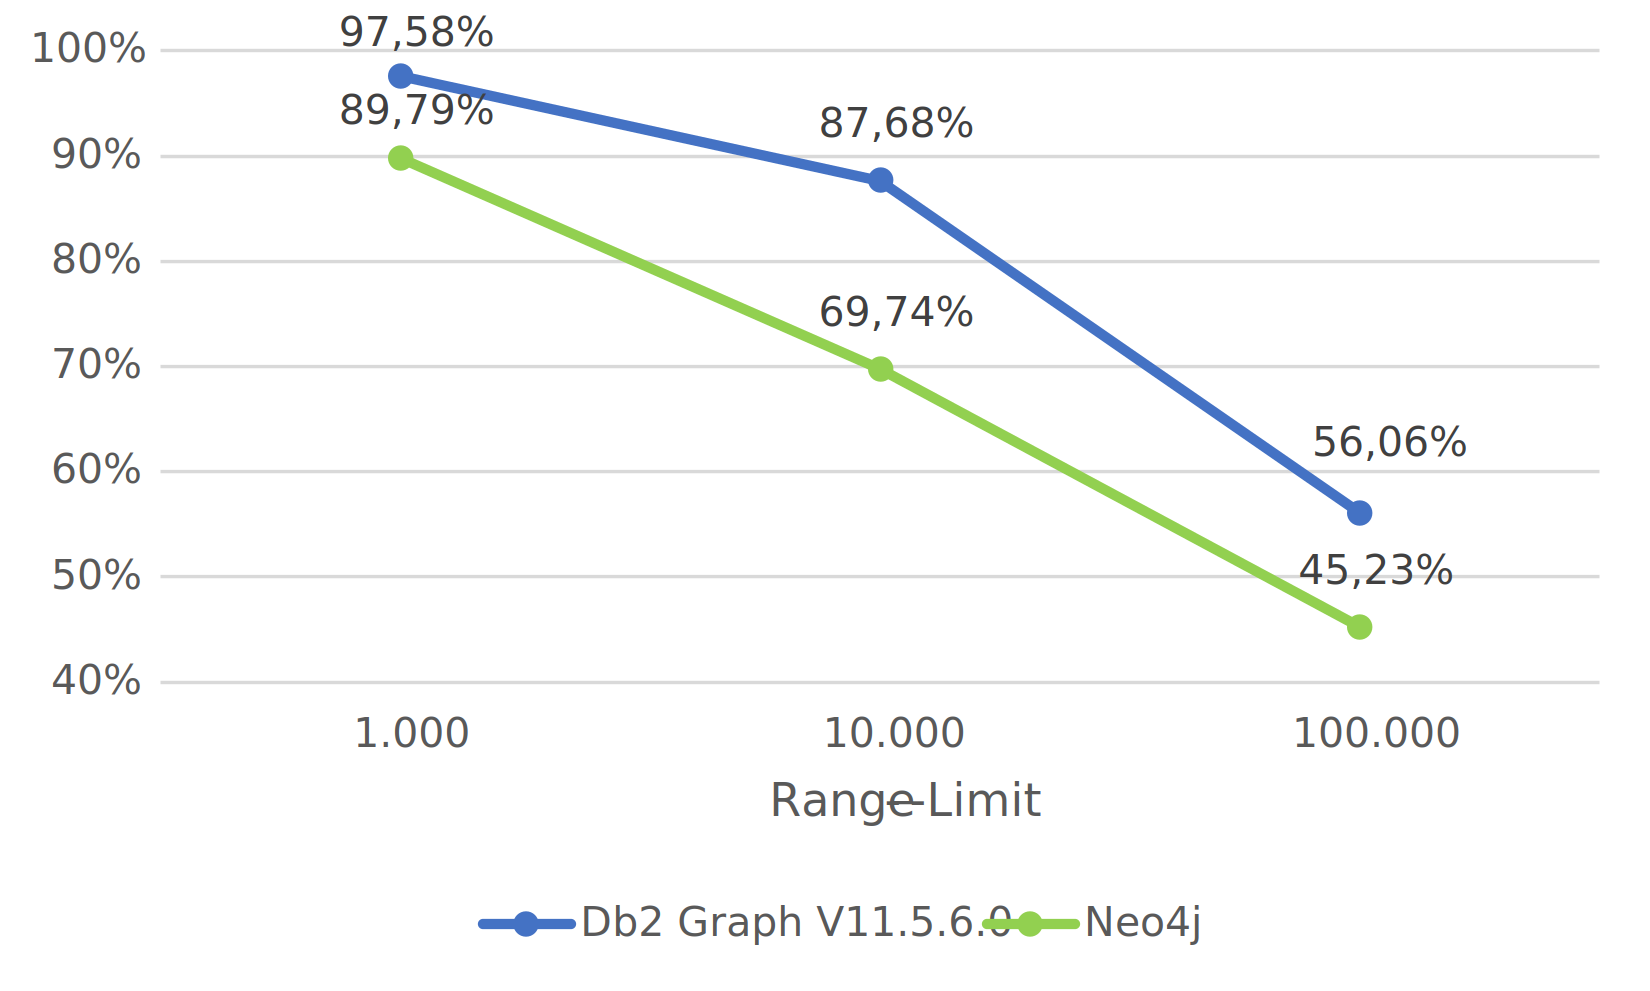
\includegraphics[width=\textwidth]{images/diagramme/limit_relative_durchsatz_real_10m.pdf}
    \caption{Linkbench-10M-Real Durchsatz gemessen an getLinkList(100)}
    \label{fig:einbruch:durchsatz:10m}
\end{figure}

\begin{figure}[!ht]
    \centering
    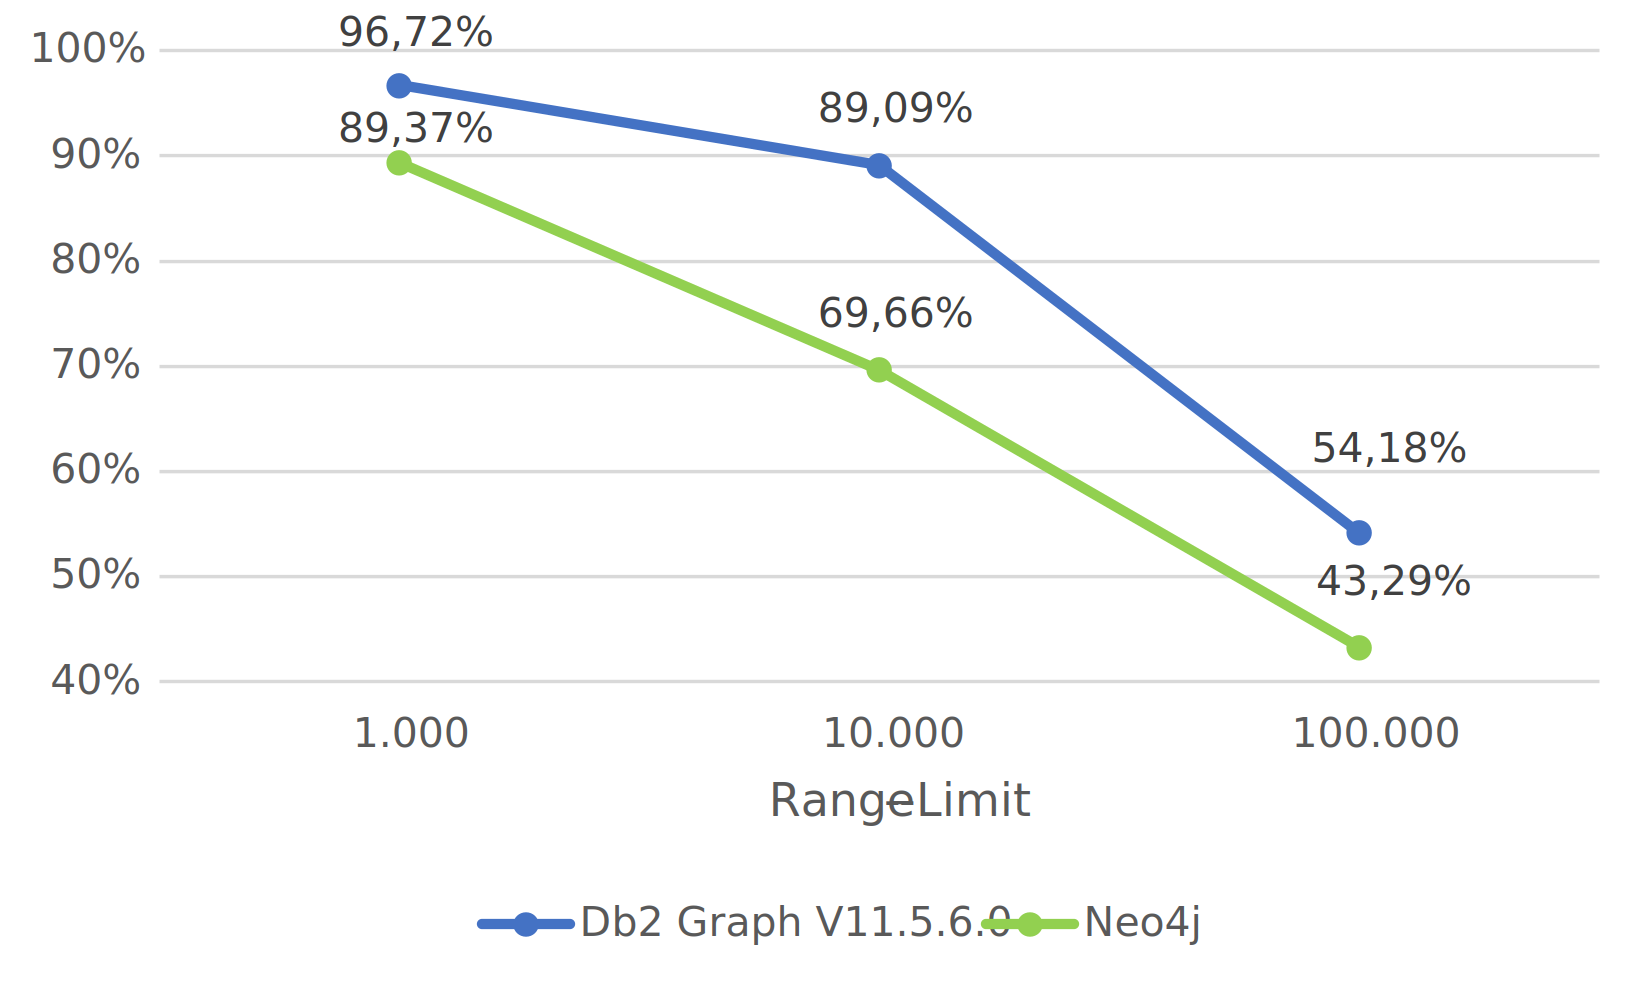
\includegraphics[width=\textwidth]{images/diagramme/limit_relative_durchsatz_real_100m.pdf}
    \caption{Linkbench-100M-Real Performance gemessen an getLinkList(100)}
    \label{fig:einbruch:durchsatz:100m}
\end{figure}

Schlussendlich kann basierend auf \autoref{fig:einbruch:durchsatz:10m} und \autoref{fig:einbruch:durchsatz:100m} geschlussfolgert werden, dass der Performance Einbruch beim Umgang mit größeren Ergebnismengen nicht nur absolut bei Neo4j größer ausfällt, sondern auch verhältnismäßig.

\subsection{Einfluss der Datensatzgröße}
Im Rahmen dieses Abschnitts wird genauer untersucht, wie groß d

\subsection{Vergleich zwischen den Verteilungen}

\subsection{Ressourcenauslastung}

\todo{Auf Ressourcenauslastung verweisen.}

\listoftodos